\pdfminorversion=7
\documentclass[10pt,journal]{IEEEtran}

\usepackage{amsmath,amssymb,amsfonts}
\usepackage{graphicx}
\usepackage[nocompress]{cite}
\usepackage{url}
\makeatletter
\g@addto@macro\UrlBreaks{\do\-}
\makeatother
\usepackage{hyperref}
\usepackage{booktabs}
\usepackage{makecell}
\usepackage{multirow}
\usepackage{xcolor}
\usepackage{tabularray}
\usepackage{placeins}
\usepackage[ruled,vlined,linesnumbered]{algorithm2e}

\usepackage[dvipsnames]{xcolor}
% \newcommand{\zxit}[1]{\textit{#1}}
% \newcommand{\zxbf}[1]{\textbf{#1}}
% \newcommand{\zxcz}[1]{\textcolor{black}{#1}}

% \newcommand{\zxca}[1]{\textcolor{blue}{#1}}
% \newcommand{\zxcb}[1]{\textcolor{orange}{#1}}
% \newcommand{\zxcc}[1]{\textcolor{cyan}{#1}} % cerulean
% \newcommand{\zxcd}[1]{\textcolor{magenta}{#1}}
% \newcommand{\zxce}[1]{\textcolor{red}{#1}}
% \newcommand{\zxcg}[1]{\textcolor{gray}{#1}}
% \newcommand{\zxch}[1]{\textcolor{purple}{#1}} % 
% \newcommand{\zxci}[1]{\textcolor{teal}{#1}} 


% % \newcommand{\zxca}[1]{\textcolor{black}{#1}} % {\textcolor{blue}{#1}}
% % \newcommand{\zxcb}[1]{\textcolor{black}{#1}} % {\textcolor{orange}{#1}}
% % \newcommand{\zxcc}[1]{\textcolor{black}{#1}} % {\textcolor{cyan}{#1}} % cerulean
% % \newcommand{\zxcd}[1]{\textcolor{black}{#1}} % {\textcolor{magenta}{#1}}
% % \newcommand{\zxce}[1]{\textcolor{black}{#1}} % {\textcolor{red}{#1}}
% % \newcommand{\zxcg}[1]{\textcolor{black}{#1}} % {\textcolor{gray}{#1}}
% % \newcommand{\zxch}[1]{\textcolor{black}{#1}} % {\textcolor{purple}{#1}} % 
% % \newcommand{\zxci}[1]{\textcolor{black}{#1}} % {\textcolor{teal}{#1}} 


\hypersetup{
    hidelinks,
    colorlinks=true,
}

\allowdisplaybreaks

\begin{document}

\title{Preference-Aware Deep Reinforcement Learning with GP-Evolved Actions for Dynamic Workflow Scheduling in Cloud--Edge Computing}

\author{Anonymous Authors}


% \author{Zaixing~Sun, 
%         Kaixuan~Ma,
%         Bin~Wang,
%         Meng~Xu,
%         Chonglin~Gu,
%         and~Hejiao~Huang
% \thanks{~~Manuscript received *; revised *; accepted *.
% This work was supported in part by the Major Key Project of PCL, China under Grant PCL2025A13, and in part by the China Postdoctoral Science Foundation under Grant Number 2026M791634, in part by Shenzhen Science and Technology Program under Grant No. JCYJ20250604145359059, and No. ZDSY20120613125016389. (Corresponding author: Chonglin~Gu.)}
% \thanks{~~Zaixing Sun and Bin Wang are with the Department of New Networks, Pengcheng Laboratory, Shenzhen, 518066, China. E-mail: zaixing.sun@micc.hitsz.edu.cn, wangb02@pcl.ac.cn.}
% \thanks{~~Kaixuan Ma, Chonglin Gu and Hejiao Huang are with the Shenzhen Key Laboratory of Internet Information Collaboration, School of Computer Science and Technology, Harbin Institute of Technology (Shenzhen), Shenzhen, 518055, China. E-mail: m2018617714@gmail.com, guchonglin@hit.edu.cn, huanghejiao@hit.edu.cn.}
% \thanks{~~Meng Xu is with Beijing Key Laboratory of Lightweight Intelligent System, Beijing Institute of Technology, Beijing, 100081, China. E-mail: mengxu@bit.edu.cn.}
% }

\maketitle


\begin{abstract}
Online workflow scheduling in heterogeneous Cloud--Edge systems must allocate
resources before future workflow arrivals are known. Resource choices have
state-dependent effects on both workflow tardiness and energy consumption.
Edge Nodes avoid Cloud provisioning and reduce wide-area communication delays
but have limited capacity, whereas Cloud
Servers provide elastic and powerful computing capacity but incur additional
provisioning and communication overheads. Their relative benefits further
depend on task characteristics, workflow dependencies, and energy efficiency.
Therefore, scheduling policies must adapt to user-requested objective
trade-offs and evolving system states. Genetic
programming (GP) hyper-heuristics have demonstrated effectiveness in evolving
resource-selection rules for dynamic workflow scheduling, but usually apply
them as fixed policies. Deep reinforcement learning enables adaptive control,
yet directly treating a variable set of feasible resources as actions while
handling multiple preferences complicates policy learning. We propose
Preference-Aware Risk-Stratified Genetic Programming-assisted Deep
Reinforcement Learning (PRS-GPDRL). Cooperative coevolution genetic programming (CCGP)
first evolves coupled task-sequencing and resource-selection rules. Quality- and
behavior-aware filtering then retains a compact resource-selection rule pool
from the final CCGP archive. Each retained rule is paired with base and risk
modes. A multi-objective double deep Q-network then selects a rule-mode action
under the requested preference at each allocation decision. Across 12 scenarios
(30 independent runs each), PRS-GPDRL achieves the best average ranks for
hypervolume (HV) and inverted generational distance (IGD), with ranks of 1.406
and 1.486, respectively, and
statistically outperforms or matches CCGP in 11 scenarios per metric. Gains are
clearest on small- and medium-scale sets, and selected large-scale scenarios show
additional HV gains. Behavioral, ablation, and diagnostic results support
preference-dependent rule selection, risk-stratified adjustment, and the focus
on resource selection.
\end{abstract}

\begin{IEEEkeywords}
Cloud--Edge computing, dynamic workflow scheduling, genetic programming,
deep reinforcement learning, multi-objective optimization.
\end{IEEEkeywords}

\section{Introduction}
\label{Sec: introduction}
\IEEEPARstart{C}{loud--Edge} computing provides a heterogeneous execution environment for workflow applications by combining latency-proximate Edge Nodes with elastic Cloud Servers. These applications include scientific workflows, data analytics pipelines, Internet of Things services, and emerging artificial intelligence agent orchestration services \cite{Li2026,Bouabdallah2024,Coleman2022WfCommons,Gartner2025AgenticAI}. Many workflow applications are represented as directed acyclic graphs (DAGs), where tasks are constrained by precedence and data dependencies \cite{Li2026,Bouabdallah2024,Coleman2022WfCommons}. As workflows arrive dynamically, a scheduler must order ready tasks and allocate heterogeneous resources without knowing future arrivals. Energy consumption has also become an important system-level constraint. Data centers consumed around 415~TWh worldwide in 2024, accounting for about 1.5\% of global electricity demand, and their share of metered electricity consumption reached 23\% in Ireland in 2025 \cite{IEA2025EnergyAI,CSO2026DataCentres}. These trends make dynamic workflow scheduling in Cloud--Edge computing a key problem for improving quality of service while controlling resource use and energy consumption.

The main difficulty is that each resource allocation must be evaluated in the current workflow and resource state, because its effects may propagate beyond the task being assigned. \emph{First}, workflow dependencies make task completion times affect downstream execution. The finish time of a task determines when its successors can be released and may further affect workflow completion and service quality. \emph{Second}, Cloud--Edge heterogeneity creates different trade-offs between latency and capacity. Edge Nodes can shorten data paths and avoid Cloud provisioning, but their computing capacity is limited. Cloud Servers provide elastic capacity, but may introduce additional communication and provisioning overheads. \emph{Third}, the CPU-sharing model considered in this paper couples the progress of tasks running on the same resource. Container virtualization provides a practical execution substrate for workflow tasks \cite{Ranjan2020}, and modern platforms support runtime resource adjustment through mechanisms such as Kubernetes in-place resource resizing and Docker CPU share or quota updates \cite{Kubernetes2026Resize,DockerUpdate2026,DockerResourceConstraints2026}. In our model, multiple tasks may execute on one resource and share its CPU capacity. Assigning a new task changes the running-task set, so the CPU allocated to CPU-sensitive tasks may be recomputed. As a result, the allocation may change remaining execution times, successor release times, resource active duration, and energy consumption. Therefore, an effective scheduler should consider dependency-driven task urgency, heterogeneous resource effects, and runtime CPU allocation when making online decisions. In a multi-objective setting, resource selection should also adapt to the requested tardiness--energy preference.

Many dynamic workflow scheduling studies use manual rules or genetic programming (GP) hyper-heuristics to support online decisions. Manual rules often combine task priorities, sub-deadlines, resource reuse, cost or energy estimates, and candidate filtering to guide task sequencing and resource allocation \cite{ohds,rmes,li2024,lou2023,lwff}. Their scheduling logic is explicit, but their performance depends on expert knowledge in selecting and combining task, workflow, and resource attributes. When the execution environment, resource model, workload pattern, or objective preference changes, these rules often require redesign or careful adjustment. GP hyper-heuristics reduce this manual design effort by automatically evolving priority rules from selected attributes. Instead of searching for one schedule for one instance, GP searches the heuristic space and produces rules that can be applied to new dynamic instances. GP has been used to evolve single-tree, multi-objective, multi-tree, dual-tree, and cooperative rules for task sequencing, resource selection, and related workflow scheduling decisions \cite{escott2020gphh,yu2022mogp,xu2023mtgp,sun2024mtgp,yang2025dtgp,ccgp}. However, most GP hyper-heuristic methods deploy one evolved heuristic or a fixed set of cooperating rules throughout an online scheduling run. They do not decide online which evolved resource-selection rule is more suitable for the current task urgency, resource availability, CPU allocation, and objective preference.

Deep reinforcement learning (DRL) offers a way to learn online selection policies from scheduling experience, but two issues must be addressed in this setting. \emph{First}, directly using feasible resources as actions is difficult for dynamic workflow scheduling in Cloud--Edge computing because the action set changes with task requirements, resource availability, and on-demand Cloud provisioning \cite{jayanetti2022,xiao2025,gates}. Rule-assisted DRL avoids this issue by using scheduling rules as fixed actions, where the selected rule ranks feasible candidates at the current decision point. Existing rule-assisted studies use manual rules or GP-evolved rules in dynamic scheduling \cite{liu2022rules,xu2024niching,zhao2025tdrl}, and GP-evolved actions have also been applied to dynamic Fog workflow scheduling \cite{he2026evolved}. However, these studies mainly address single-objective or fixed-objective settings, and rule sets based on manual rules still depend on expert design. \emph{Second}, different users or scenarios may require different tardiness--energy trade-offs. Multi-objective reinforcement learning (MORL) and Pareto set learning can condition decisions on preferences \cite{roijers2013morl,hayes2022morl,abels2019morl,yang2019morl,lin2022psl,xu2026pslgp}. However, they do not provide a rule-mode action design that combines a compact pool of GP-evolved resource-selection rules with preference-aware online selection. This gap motivates combining GP-based generation of complementary resource-selection rules with DRL-based preference-aware online selection.

To address these gaps, this paper proposes Preference-Aware Risk-Stratified Genetic Programming-assisted Deep Reinforcement Learning (PRS-GPDRL). Cooperative coevolution genetic programming (CCGP) is used to generate a multi-objective archive of scheduling heuristics. A quality- and behavior-aware extraction procedure then constructs a compact pool of complementary resource-selection rules from this archive. Each retained resource-selection rule is paired with a base mode and a risk mode. The base mode follows the selected GP rule, while the risk mode adds a bounded preference-aware local correction. Pairing the retained rules with these two modes gives a fixed rule-mode action space for the DRL agent. A multi-objective double deep Q-network (DDQN) learns to select rule-mode actions according to the current system state and requested preference.
The main contributions are as follows:
\begin{itemize}
    \item We establish a CCGP-to-DRL knowledge interface that extracts high-quality and behaviorally complementary resource-selection rules from a CCGP archive. Pairing the compact rule pool with base and risk modes converts these executable heuristics into a fixed rule-mode action space that ranks the variable feasible-resource set at each allocation decision.

    \item We develop two-level adaptive resource selection through risk-stratified action augmentation. A selected GP rule supplies the global ranking direction, while the risk mode conditionally applies a bounded local correction using the current state and requested preference. Feature-wise linear modulation (FiLM) conditioning, vector-valued action costs, and augmented weighted Tchebycheff scalarization enable one DDQN to serve different tardiness--energy preferences.

    \item Across 12 dynamic scheduling scenarios, with 30 independent runs conducted per scenario, PRS-GPDRL obtains the best average ranks for hypervolume (HV) and inverted generational distance (IGD), with ranks of 1.406 and 1.486, respectively. It is statistically better than or comparable to CCGP in 11 of 12 scenarios and to GATES and LWFF in at least 11 of 12 scenarios for each metric. The clearest advantages occur on small- and medium-scale workflow sets, with additional HV gains in selected large-scale scenarios.

    \item Behavioral analyses show preference-aligned changes at the outcome, rule, and mode levels: objective values respond to the requested preference, online selection migrates between energy- and tardiness-oriented rule roles, and local risk correction is activated selectively. Ablation and diagnostic results further distinguish the contributions of complementary rule coverage, preference-dependent representation, local correction, and task sequencing.
\end{itemize}

\section{Related Work}
\label{Sec: related work}

\subsection{Rule-Based Dynamic Workflow Scheduling}

Dynamic workflow scheduling in cloud, fog, and Cloud--Edge environments has been studied under deadline, cost, energy, and utilization objectives \cite{ohds,rmes,li2024,lou2023,lwff}. Manual rules and constructive methods remain important because they can be directly applied during online scheduling. Fan et al.~\cite{ohds} proposed Online Hybrid Dynamic Scheduling (OHDS), which integrates task merging, sub-deadline assignment, hybrid scheduling of multiple workflows, dynamic priority adjustment, and virtual machine migration based on CPU utilization. Sun et al.~\cite{rmes} proposed Real-time Multi-workflow Energy-efficient Scheduling (RMES) for container-based clouds, where sub-deadlines, container-machine affinity, resource reuse, and rescheduling of remaining tasks are used for energy-efficient real-time scheduling. Fard et al.~\cite{lwff} proposed Least Waste Fast First (LWFF) for microservice placement, using CPU and memory requests to improve multi-resource utilization and throughput. These methods provide clear scheduling mechanisms for their target resource models and objectives. Although some of them update priorities or reschedule tasks during execution, the priority and scoring rules are still specified by design. Therefore, they provide limited support for changing the scheduling behavior online when workload conditions or objective preferences vary.

Learning-based methods learn scheduling policies or candidate evaluations from data or simulation experience. DRL and multi-agent DRL have been used to address time--energy scheduling, multi-objective resource allocation, and collaborative workflow offloading in Cloud--Edge environments \cite{jayanetti2022,zhang2024,xiao2025}. GATES uses graph attention to encode variable ready-task and virtual-machine states, and trains the allocation policy through an evolution strategy \cite{gates}. Reinforcement learning-based hyper-heuristics have also been studied for energy-efficient cloud workflow scheduling \cite{li2025qphh}. These studies improve adaptive decision making for dynamic workflow scheduling, but their learned components mainly produce direct allocation policies, resource scores, or selections among predefined low-level heuristics. They do not focus on online deployment of a pool of evolved resource-selection rules.

GP hyper-heuristics address rule generation by searching for executable priority rules. Escott et al.~\cite{escott2020gphh} introduced GP hyper-heuristics for dynamic cloud workflow scheduling to generate rules from a richer set of task and resource attributes. Yu et al.~\cite{yu2022mogp} extended this idea to multi-objective dynamic workflow scheduling. Xu et al.~\cite{xu2023mtgp}, Sun et al.~\cite{sun2024mtgp}, and Yang et al.~\cite{yang2025dtgp} further studied GP rule generation for fog, multi-cloud, and cloud workflow scheduling with different rule representations. Sun et al.~\cite{ccgp} proposed CCGP for dynamic joint workflow scheduling and container scaling in Cloud--Fog computing. CCGP evolves task-sequencing, resource-selection, and container-scaling rules in cooperating subpopulations. These studies show that GP can automatically discover scheduling rules for dynamic workflow environments. However, the evolved heuristic or cooperating rule set is normally fixed before online execution. Thus, GP can provide useful rules, but it does not decide online which resource-selection rule should be applied under the current workflow state and objective preference.

Rule-assisted DRL addresses online rule selection by defining actions over scheduling rules rather than over a changing set of candidate jobs or resources. Liu et al.~\cite{liu2022rules} used manual dispatching rules as actions for DRL in dynamic flexible job-shop scheduling. This indirect action representation avoids direct action definitions over variable candidate sets, but its performance is limited by the manual rule library. Xu et al.~\cite{xu2024niching} replaced manual actions with heuristics evolved by niching GP, and the behaviorally different heuristics are then used as DRL actions. Zhao et al.~\cite{zhao2025tdrl} studied GP-assisted DRL for dynamic flexible job-shop scheduling, and He et al.~\cite{he2026evolved} applied GP-evolved actions to dynamic fog workflow scheduling. These studies are closely related to the rule-action design in this paper. However, they mainly address dynamic job-shop scheduling or fixed-objective workflow scheduling. They do not directly consider preference-aware online selection from a compact resource-selection rule pool extracted from a multi-objective GP archive for dynamic workflow scheduling in Cloud--Edge computing.

\subsection{Preference-Aware Multi-Objective Learning}

MORL studies sequential decision making with vector-valued returns and different objective trade-offs \cite{roijers2013morl,hayes2022morl}. One line learns multiple policies or a continuous Pareto manifold to cover different non-dominated regions \cite{vanmoffaert2014pareto,parisi2016pareto}. Another line conditions a shared value function or policy on the requested preference. For example, Abels et al.~\cite{abels2019morl} conditioned deep Q-networks on dynamic objective weights, and Yang et al.~\cite{yang2019morl} learned a generalized policy for different preferences. Recent MORL studies further improve preference control and adaptation in learned policies \cite{reymond2022pcn,wu2026e2morl,yang2025pcrl}. These methods provide useful preference representations for multi-objective decision making. However, their focus is preference-aware policy learning rather than scheduling-rule generation and online rule deployment.

Preference-aware ideas have also been introduced into evolutionary multi-objective optimization. Pareto set learning maps a preference vector to an approximate Pareto solution through scalarization-based training \cite{lin2022psl}. Xu et al.~\cite{xu2026pslgp} proposed Pareto Set Learning GP (PSLGP) for multi-objective dynamic scheduling. PSLGP uses the preference as an input to a single GP heuristic, reducing the need to manage many heuristics for different Pareto regions. This line shows that preferences can guide evolved decision rules. The remaining issue for this paper is different: how to use DRL to select online among multiple GP-evolved resource-selection rules while the feasible resource set and workflow state change over time. This motivates preference-aware online deployment of complementary GP-evolved resource-selection rules for dynamic workflow scheduling in Cloud--Edge computing.


\section{Problem Modeling}
\label{Sec: problem modeling}

We consider a heterogeneous Cloud--Edge computing environment for dynamic workflow execution. Let $R=C\cup E$ be the set of computing resources, where $C$ and $E$ denote the sets of Cloud Servers and Edge Nodes, respectively. Each resource $r\in R$ is modeled as a virtual machine (VM) with CPU capacity $\Gamma^c(r)$. Edge Nodes form a fixed resource pool with limited capacity, whereas Cloud Servers can be provisioned on demand. Tasks are packaged as containers and deployed to selected resources. A resource can run multiple containers simultaneously, but the total CPU allocated to the running containers cannot exceed the CPU capacity of the resource at any moment. A container is the minimum execution unit and executes one task at a time. The scheduling model treats CPU capacity as the adjustable resource.
Let $B_{\mathrm{edge}}$ and $L_{\mathrm{edge}}$ be the bandwidth and latency for communications within the Edge tier, respectively. Let $B_{\mathrm{cloud}}$ and $L_{\mathrm{cloud}}$ be the bandwidth and latency for communications involving Cloud Servers, respectively. Each resource has static power and CPU-based dynamic power. Static power $p^s(r)$ consists of base power $p^b(r)$ and CPU-based idle power $p^{ic}(r)$, where $p^s(r)=p^b(r)+p^{ic}(r)$. Dynamic power is defined as the difference between CPU full power and CPU idle power, namely $p^{dc}(r)=p^{fc}(r)-p^{ic}(r)$. The energy consumption of both Cloud Servers and Edge Nodes is considered in this work.

Let $\mathcal{W}$ be the set of workflow applications. Each workflow $\omega\in\mathcal{W}$ contains a task set $A(\omega)$. The arrival time, weight, and deadline of workflow $\omega$ are $\rho^a(\omega)$, $\rho^w(\omega)$, and $\rho^d(\omega)$, respectively. Each task $\alpha\in A(\omega)$ is represented by $\{\phi(\alpha),\tau^l(\alpha),\mu^c(\alpha),A^{pre}(\alpha),A^{suc}(\alpha)\}$, where $\phi(\alpha)\in\{0,1\}$ denotes the task category, $\tau^l(\alpha)$ is its CPU workload, $\mu^c(\alpha)$ is its minimum CPU requirement, and $A^{pre}(\alpha),A^{suc}(\alpha)\subseteq A(\omega)$ are its predecessor and successor task sets, respectively. Let $d(\alpha_1,\alpha_2)$ be the data transferred from task $\alpha_1$ to its successor task $\alpha_2\in A^{suc}(\alpha_1)$. The execution time of a task depends on its category and allocated CPU capacity. Tasks are divided into two categories.
\begin{itemize}
    \item $\phi(\alpha)=0$.
    The allocated CPU must meet the task's minimum CPU requirement, but allocating more CPU does not reduce its execution time. Such tasks are CPU-insensitive.
    \item $\phi(\alpha)=1$.
    The allocated CPU must meet the task's minimum CPU requirement, and a larger allocation can reduce its execution time. Such tasks are CPU-sensitive.
\end{itemize}

We formulate dynamic workflow scheduling with deadline constraints as a bi-objective optimization problem. The objectives are to minimize system-oriented total energy consumption and workflow-oriented total weighted tardiness under the following scheduling and resource constraints:
\begin{itemize}
    \item No task can be executed until all its predecessor tasks have been completed.
    \item Each task must be executed by a container whose allocated CPU satisfies the task's minimum CPU requirement.
    \item Each resource can deploy and run multiple containers simultaneously, but the sum of their allocated CPU capacities cannot exceed the resource's CPU capacity at any moment.
\end{itemize}

We model dynamic workflow scheduling as a discrete-event control process. Let $\mathcal{T}$ be the set of decision points, and let $t\in\mathcal{T}$ be a specific decision point. Decision points typically correspond to moments when the system state changes, such as when a workflow is submitted, a task becomes ready, a task starts execution, or a task completes. Let $x^s(\alpha)$ and $x^f(\alpha)$ be the execution start time and execution finish time of task $\alpha$, respectively. Let $y(\alpha)\in R$ be the assigned resource of task $\alpha$ in the schedule. Let $\nu^c(\alpha,t)$ be the CPU allocated to the container executing task $\alpha$ at time $t$.

The problem can then be formulated as
\begin{align}
    \min~ & \mathbb{E} =
    \sum_{r\in R}\int_{\mathcal{T}} P(r,t)dt,
    \label{Eq: Objective Energy} \\
    \min~ & \mathbb{T} =
    \sum_{\omega\in\mathcal{W}}
    \rho^w(\omega)\times
    \max\left\{
    0,
    \max\limits_{\alpha\in A(\omega)}
    \left\{x^f(\alpha)\right\}
    -\rho^d(\omega)
    \right\},
    \label{Eq: Objective Tardiness} \\
    s.t.:~&
    x^s(\alpha)\geq \rho^a(\omega),
    ~\forall\ \omega\in\mathcal{W},\alpha\in A(\omega),
    \label{Eq: Arrival time constraint}\\
    &
    x^f(\alpha_1)
    +x^c(\alpha_1,\alpha_2)
    +x^l(\alpha_2) \notag\\
    &\qquad
    \leq x^s(\alpha_2),
    ~\forall\alpha_2\in A^{suc}(\alpha_1),
    \label{Eq: Dependency constraint}\\
    &
    \begin{cases}
    x^f(\alpha)-x^s(\alpha)
    =
    \dfrac{\tau^l(\alpha)}{\mu^c(\alpha)},
    ~\hfill \phi(\alpha)=0,\\[6pt]
    \displaystyle
    \int_{x^s(\alpha)}^{x^f(\alpha)}
    \nu^c(\alpha,t)dt
    =
    \tau^l(\alpha),
    ~\hfill \phi(\alpha)=1.
    \end{cases}
    \label{Eq: Start-Finish time}\\
    &
    \nu^c(\alpha,t)\geq \mu^c(\alpha),
    ~\hfill \forall t\in\mathcal{T},
    \label{Eq: task requirement constraint}\\
    &
    \sum_{\alpha\in A_r(t)} \nu^c(\alpha,t)
    \leq \Gamma^c(r),
    ~\hfill \forall r\in R,\forall t\in\mathcal{T},
    \label{Eq: resource constraint}\\
    &
    x^l(\alpha)=
    \begin{cases}
    L_{\mathrm{edge}}, ~\hfill y(\alpha)\in E,\\
    L_{\mathrm{cloud}}, ~\hfill y(\alpha)\in C.
    \end{cases}
    \label{Eq: task latency}\\
    &
    x^c(\alpha_1,\alpha_2)=
    \begin{cases}
    0, ~\hfill y(\alpha_1)=y(\alpha_2),\\
    \begin{aligned}
        &\dfrac{d(\alpha_1,\alpha_2)}{B_{\mathrm{edge}}},
        ~\hfill y(\alpha_1)\neq y(\alpha_2),\\
        &~~~~~~~~~~~~~y(\alpha_1),y(\alpha_2)\in E,
    \end{aligned}\\
    \dfrac{d(\alpha_1,\alpha_2)}{B_{\mathrm{cloud}}},
    ~\hfill \text{otherwise}.
    \end{cases}
    \label{Eq: communication time between tasks}
\end{align}

The CPU allocation of containers is updated whenever a task starts or completes on a resource. Given the assigned resources $y(\alpha)$, the CPU allocation at time $t$ is determined by the running task set on each resource.
Let $A_r(t)$ be the set of running tasks on resource $r$ at time $t$, i.e.,
\begin{equation}
    A_r(t)=
    \{\alpha\mid y(\alpha)=r,~x^s(\alpha)\leq t<x^f(\alpha)\}.
    \label{Eq: running set}
\end{equation}
% Let $S_r(t)= \{\alpha\in A_r(t)\mid \phi(\alpha)=1\}$ be the set of CPU-sensitive running tasks on resource $r$ at time $t$.
% \begin{equation}
%     S_r(t)= \{\alpha\in A_r(t)\mid \phi(\alpha)=1\}.
%     \label{Eq: sensitive set}
% \end{equation}
The remaining CPU capacity after satisfying the minimum CPU requirements of all running tasks is
\begin{equation}
    \Gamma_{\mathrm{rem}}^c(r,t)=
    \Gamma^c(r)
    -
    \sum\nolimits_{\beta\in A_r(t)}
    \mu^c(\beta).
    \label{Eq: remaining cpu}
\end{equation}
Let $S_r(t)= \{\alpha\in A_r(t)\mid \phi(\alpha)=1\}$ be the set of CPU-sensitive running tasks on resource $r$ at time $t$.
For each running task $\alpha\in A_r(t)$, the CPU allocation is calculated as
\begin{equation}
    \nu^c(\alpha,t)=
    \begin{cases}
        \mu^c(\alpha),
        & \phi(\alpha)=0,\\[4pt]
        \mu^c(\alpha)+
        \dfrac{\Gamma_{\mathrm{rem}}^c(r,t)}{|S_r(t)|},
        & \phi(\alpha)=1.
    \end{cases}
    \label{Eq: cpu allocation}
\end{equation}
Thus, CPU-insensitive tasks use their minimum CPU requirements, while CPU-sensitive tasks equally share the remaining CPU capacity.
The CPU utilization of resource $r$ at time $t$ is
\begin{equation}
    U^c(r,t)=
    \frac{
    \sum_{\alpha\in A_r(t)}
    \nu^c(\alpha,t)}
    {\Gamma^c(r)}.
    \label{Eq: Utilization at time t}
\end{equation}
The instantaneous power consumption of resource $r$ is modeled as
\begin{equation}
    P(r,t)=
    p^s(r)+p^{dc}(r)\left(U^c(r,t)\right)^3.
    \label{Eq: power at time t}
\end{equation}
The above equations hold for $\forall\ \omega\in\mathcal{W}$, $\forall\ \alpha,\alpha_1,\alpha_2\in A(\omega)$, $\forall\ r\in R$, and $\forall t\in\mathcal{T}$ when the corresponding quantities are defined. Eqs.~\eqref{Eq: Objective Energy} and~\eqref{Eq: Objective Tardiness} are the two objectives considered in this work. Eq.~\eqref{Eq: Objective Energy} gives the total energy consumption by integrating the instantaneous power $P(r,t)$ over all Cloud Servers and Edge Nodes. Eq.~\eqref{Eq: Objective Tardiness} gives the workflow-oriented total weighted tardiness. Constraint~\eqref{Eq: Arrival time constraint} ensures that a workflow cannot be executed until it is submitted, and thus the scheduler has no information about that workflow before its arrival. Constraint~\eqref{Eq: Dependency constraint} enforces workflow precedence and data transfer dependencies. A task can start only after all of its immediate predecessors have finished and their output data have arrived. Eq.~\eqref{Eq: Start-Finish time} defines the execution time of the two task categories, ensuring that each task $\alpha$ completes workload $\tau^l(\alpha)$ during $[x^s(\alpha),x^f(\alpha)]$ under the corresponding CPU allocation. Constraint~\eqref{Eq: task requirement constraint} ensures that the CPU allocation of each running task satisfies its minimum CPU requirement. Constraint~\eqref{Eq: resource constraint} ensures that the total CPU allocated to running tasks on a resource does not exceed the resource's CPU capacity at time $t$. Eq.~\eqref{Eq: task latency} defines the access latency $x^l(\alpha)$ according to whether task $\alpha$ is assigned to an Edge Node or a Cloud Server. Eq.~\eqref{Eq: communication time between tasks} gives the communication time between task $\alpha_1$ and its successor $\alpha_2$ according to their assigned resources.
Eqs.~\eqref{Eq: running set}-\eqref{Eq: cpu allocation} define the elastic CPU sharing rule. Eq.~\eqref{Eq: running set} gives the set of running tasks on resource $r$. Eq.~\eqref{Eq: remaining cpu} calculates the remaining CPU capacity after the minimum CPU requirements of all running tasks have been satisfied. Eq.~\eqref{Eq: cpu allocation} then assigns the minimum CPU requirement to each CPU-insensitive task and equally divides the remaining CPU capacity among CPU-sensitive tasks. Eq.~\eqref{Eq: Utilization at time t} gives the CPU utilization of resource $r$ at time $t$. Eq.~\eqref{Eq: power at time t} models the instantaneous power consumption of resource $r$, which consists of static power $p^s(r)$ and CPU-based dynamic power that scales cubically with CPU utilization. For on-demand Cloud Servers, the power model is evaluated only over recorded utilization intervals of provisioned resources. Unprovisioned Cloud Servers do not contribute to the energy integral in Eq.~\eqref{Eq: Objective Energy}.

\section{The Proposed PRS-GPDRL Algorithm}
\label{Sec: PRS-GPDRL}

\subsection{Overall Framework of PRS-GPDRL}
\label{Sec: PRS-GPDRL overall}

Fig.~\ref{Fig: PRS-GPDRL framework} shows the overall framework of PRS-GPDRL, which consists of offline training and online scheduling. For each training scenario, CCGP first produces an archive of complete scheduling heuristics, each of which contains a task-sequencing rule and a resource-selection rule. Although both rules are evolved cooperatively, PRS-GPDRL constructs the DDQN action space from the resource-selection rules and uses fixed upward-rank sequencing when multiple ready tasks need to be ordered. The diagnostic comparison in Section~\ref{Sec: task sequencing design} later examines this choice by separately replacing CCGP's task-sequencing and resource-selection rules. Since the variant that replaces task sequencing is statistically comparable to CCGP in most scenarios, whereas the variant that replaces resource selection is consistently worse, PRS-GPDRL concentrates the learned action space on resource-selection rules and their modes.

The offline stage extracts a compact resource-selection rule pool $\mathcal{G}$ from the final CCGP archive. Each retained rule is paired with the base and risk modes in $\mathcal{M}$, and the resulting rule-mode action space $\mathcal{A}$ remains fixed while the feasible resource set varies at runtime. A multi-objective DDQN is trained to select actions from $\mathcal{A}$ according to the task attributes, feasible resource attributes, and preference weights.

In online scheduling, fixed upward-rank sequencing is used only when multiple tasks are ready at the same decision point \cite{Topcuoglu2002}. For the selected ready task, the trained DDQN chooses a resource-selection rule and a mode according to the current state and requested preference. The selected rule-mode action then scores the feasible resources, and the task is assigned to the resource with the minimum priority score.

\begin{figure}[!t]
\centering
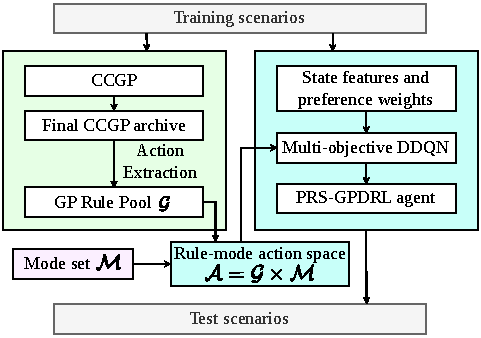
\includegraphics[width=.88\linewidth]{figures/framework.pdf}
\caption{Overall framework of PRS-GPDRL.}
\label{Fig: PRS-GPDRL framework}
\end{figure}

\subsection{CCGP Training and Action Extraction}
\label{Sec: CCGP action extraction}

\textbf{CCGP training.} CCGP cooperatively evolves task-sequencing and resource-selection rules in two subpopulations. Individuals from the two subpopulations are paired to form complete scheduling heuristics, which are evaluated on energy consumption and weighted tardiness and recorded in the archive set ($AS$). Until the stopping criterion is met, CCGP updates the two subpopulations by elitism, reproduction, crossover, and mutation. At the final generation, duplicate solutions are removed from $AS$, and the first non-dominated front is retained as the source of resource-selection rules for PRS-GPDRL.

\textbf{Rule representation.} Each GP rule is a tree-based priority expression whose terminals provide scheduling attributes and whose function nodes combine them into priority scores. Task-sequencing and resource-selection rules use different terminal subsets but share the same function set. Table~\ref{Table:scheduling-attributes} summarizes the terminals used by the GP rules and the attributes used by the DDQN state encoder. The DDQN state uses task, feasible-resource, and preference attributes, so its input is consistent with the information used by the rule-mode actions. Further details of CCGP training and terminal-value computation are given in~\cite{ccgp}.

\begin{table}[!t]
\centering
\caption{Terminal, function, and state-encoder attributes used by PRS-GPDRL.}
\label{Table:scheduling-attributes}
% \scriptsize
\setlength{\tabcolsep}{.8pt}
% \renewcommand{\arraystretch}{0.94}
\begin{tabular}{@{}cp{0.63\columnwidth}cc@{}}
% \hline
\toprule
Notation & Description & GP & DDQN \\
\midrule
$\mathsf{CAT}$   & Category of a task. & T & T \\
$\mathsf{SD}$    & Sub-deadline of a task. & T & T \\
$\mathsf{ET}$    & Execution time of a task on a reference resource. & T & T \\
$\mathsf{CPUA}$  & Minimum CPU requirement of a task. & T & T \\
$\mathsf{WT}$    & Weight of a workflow. & T & T \\
$\mathsf{UR}$    & Task upward-rank value. & T & T \\
$\mathsf{NSA}$   & Number of direct successors of a task. & T & T \\
$\mathsf{NPA}$   & Number of direct predecessors of a task. & T & -- \\
$\mathsf{NKQ}$   & Number of tasks in the ready queue. & T & -- \\
$\mathsf{TETQ}$  & Total $\mathsf{ET}$ of tasks in the ready queue. & T & -- \\
$\mathsf{NRA}$   & Number of remaining tasks in a workflow. & T & T \\
$\mathsf{TETRA}$ & Total $\mathsf{ET}$ of remaining workflow tasks. & T & T \\
$\mathsf{VCT}$   & Average communication time for a task. & T & T \\
% \midrule
\cmidrule(lr){1-4}
$\mathsf{NEW}$   & Whether the resource is newly created. & -- & R \\
$\mathsf{WAIT}$  & Waiting time before the task starts on a resource. & R & R \\
$\mathsf{ETAR}$  & Minimum execution time of a task on a resource. & R & R \\
$\mathsf{CRCPU}$ & Current remaining CPU of a resource. & R & R \\
$\mathsf{ST}$    & Slack time of a task on a resource. & R & R \\
$\mathsf{STPR}$  & Static power of a resource. & R & R \\
$\mathsf{DPR}$   & Dynamic power of a resource. & R & R \\
$\mathsf{NTR}$   & Number of tasks on a resource. & R & R \\
$\mathsf{NKW}$   & Number of scheduled tasks from the same workflow in the Cloud or
Edge tier. & R & R \\
$\mathsf{CPUR}$  & CPU capacity of a resource. & R & R \\
$\mathsf{CTR}$   & Communication time of a task on a resource. & R & R \\
% \midrule
\cmidrule(lr){1-4}
$w_T$ & Preference weight for weighted tardiness. & -- & P \\
$w_E$ & Preference weight for energy consumption. & -- & P \\
\midrule
Function set & $+$, $-$, $\times$, protected~/, Max, and Min. & T/R & -- \\
\bottomrule
\multicolumn{4}{p{0.95\linewidth}}{In the GP column, T and R denote task-sequencing and resource-selection rule terminals. In the DDQN column, T, R, and P denote task, feasible resource, and preference attributes, respectively.}
\end{tabular}
\vspace{-1em}
% \end{tabular}
% \vspace{1pt}

% \parbox{\columnwidth}{\scriptsize In the GP column, T and R denote task- and
% resource-selection rule terminals. In the DDQN column, T, R, and P denote task,
% feasible resource, and preference attributes, respectively.}
\end{table}

\textbf{Action extraction.} After CCGP training, PRS-GPDRL constructs $\mathcal{G}$ from the first non-dominated front retained from $AS$. For a complete heuristic $i$ in this front, let $g_i$ denote its resource-selection rule. Different heuristics may contain resource-selection rules that make the same choices at representative decision points. Therefore, the extraction procedure retains rules from different regions of the validation trade-off front and removes behaviorally duplicate rules. It consists of validation evaluation, decision point sampling, behavioral representation, and anchor selection.

\textbf{Validation evaluation.} Each complete heuristic in the retained front is evaluated on a validation set of random seeds to obtain a bi-objective performance estimate for anchor selection. The validation performance is represented by the mean energy consumption and mean weighted tardiness over three independent runs. Let $S_i^{\mathrm{val}}=\widehat{\mathbb{E}}_i^{\mathrm{val}}+\widehat{\mathbb{T}}_i^{\mathrm{val}}$ denote the normalized validation score of heuristic $i$, where $\widehat{\mathbb{E}}_i^{\mathrm{val}}$ and $\widehat{\mathbb{T}}_i^{\mathrm{val}}$ are its min--max normalized validation energy and weighted tardiness, respectively. The score is used only for validation-based selection among CCGP heuristics and does not replace the final test evaluation.

\textbf{Decision point sampling.} A reference scheduling heuristic is selected from the validation-evaluated heuristics by minimizing $S_i^{\mathrm{val}}$. The reference heuristic is then executed to collect representative resource allocation decision points. At each sampled decision point, all feasible resources are recorded with their current terminal attributes. These samples provide a common set of online decision contexts for comparing the behavior of different resource-selection rules.

\textbf{Behavioral representation.} The behavior of resource-selection rule $g_i$ is measured by replaying it on the sampled decision points. At decision point $d$, the rule scores all feasible resources and selects the resource with the minimum priority score. The behavior vector of $g_i$ is
\begin{equation}
    \mathbf{b}_i = \left( \pi_i(d_1), \pi_i(d_2), \ldots, \pi_i(d_M) \right),
    \label{Eq: behavior vector}
\end{equation}
where $\pi_i(d_m)$ is the resource index selected by $g_i$ at sampled decision point $d_m$, and $M=20$ is the number of sampled decision points. In implementation, $\pi_i(d_m)$ is encoded as a resource-selection indicator vector, so tied best resources are represented as the same selected set. Rules producing identical behavior vectors are grouped together, and the rule whose complete heuristic has the lowest $S_i^{\mathrm{val}}$ is retained as the representative.

\textbf{Anchor selection.} Let $K$ denote the maximum requested size of the resource-selection rule pool. If the number of behaviorally unique rules does not exceed $K$, all representatives are retained. For the default $K=5$, the retained rules are otherwise selected from five representative positions on the validation front: the minimum-energy endpoint, a low-energy neighbor, a balanced anchor, a low-tardiness neighbor, and the minimum-tardiness endpoint. Selecting these positions preserves rules associated with different tardiness--energy trade-off regions, so that the DDQN can choose among complementary resource-selection behaviors during online scheduling. The endpoints minimize $\widehat{\mathbb{E}}_i^{\mathrm{val}}$ and $\widehat{\mathbb{T}}_i^{\mathrm{val}}$, respectively. After excluding the endpoints, each neighbor is drawn from the corresponding 5\% normalized objective band. A heuristic belongs to this band when its corresponding normalized objective value does not exceed 0.05. If the band contains too few behaviorally distinct rules, top-ranked heuristics under the same objective are also considered. Let $i_E$ and $i_T$ denote the two endpoint indices. The balanced anchor is selected by
\begin{equation}
\begin{aligned}
    S_i^{\mathrm{bal}}
    &=\max\left\{
        \widehat{\mathbb{E}}_i^{\mathrm{val}},
        \widehat{\mathbb{T}}_i^{\mathrm{val}}
      \right\}
      +0.05\left(
        \widehat{\mathbb{E}}_i^{\mathrm{val}}+
        \widehat{\mathbb{T}}_i^{\mathrm{val}}
      \right),\\
    i_{\mathrm{bal}}
    &=\arg\min_{i\notin\{i_E,i_T\}} S_i^{\mathrm{bal}}.
\end{aligned}
    \label{Eq: balanced anchor}
\end{equation}
For the $K=3$ ablation, the minimum-energy endpoint, the balanced anchor, and the minimum-tardiness endpoint are retained. If a selected rule duplicates an already retained behavior, the next behaviorally distinct rule from the same region or objective ranking is used.

For a given CCGP run $b$, the retained resource-selection rules form $\mathcal{G}=\{g_1,\ldots,g_{K_b}\}$, where $K_b\leq K$ is the actual number retained. Combining $\mathcal{G}$ with the two modes gives the rule-mode action space $\mathcal{A}$ used by the DDQN.

\subsection{Risk-Stratified Action Augmentation}
\label{Sec: risk stratified actions}

Each extracted resource-selection rule defines a priority function for ranking the feasible resources. The normalized GP score preserves the ranking behavior learned by CCGP, but the score itself is not explicitly adjusted by the requested preference. Therefore, PRS-GPDRL pairs each resource-selection rule with a \textit{base} mode and a \textit{risk} mode. The base mode uses the normalized GP score directly. The risk mode keeps the GP score as the primary ranking term and adds a bounded correction derived from the local tardiness-related and energy-related costs defined below. In this way, the DDQN can choose either the original GP ranking or its preference-aware local correction for the current decision.

Let $\mathbf{w}=(w_T,w_E)$ be the current preference vector, where $w_T$ and $w_E$ are the weights for weighted tardiness and energy consumption, respectively, and $w_T+w_E=1$. At decision point $t$, let $\mathcal{R}_t$ be the feasible resource set and let $n=|\mathcal{R}_t|$. For a selected resource-selection rule $g_i\in\mathcal{G}$, let $\hat{g}_i(r)$ denote its min--max normalized priority score for resource $r\in\mathcal{R}_t$. For all min--max normalizations in this work, if all resources have the same value, the corresponding normalized score is set to zero for all resources.

PRS-GPDRL estimates two local costs for each resource in the same feasible resource set. These costs are used to stratify feasible resources under the requested preference. For the tardiness-related local cost, let $\alpha_t$ be the current ready task at decision time $t$, let $\mathsf{SD}(\alpha_t)$ be its sub-deadline, and let $\omega$ be the workflow containing $\alpha_t$. For resource $r$, let $t_{\alpha_t,r}^{\mathrm{ava}}$ be the actual available time for assigning $\alpha_t$ to $r$. To evaluate this feasible assignment, $\alpha_t$ is temporarily assigned to $r$ at $t_{\alpha_t,r}^{\mathrm{ava}}$, and CPU allocation is updated according to Eq.~\eqref{Eq: cpu allocation}. Let $\hat{x}_{\alpha_t,r}^{f}$ be the estimated finish time of $\alpha_t$ under this temporary assignment. The local cost combines the estimated time from the current decision point to task completion with the workflow-weighted sub-deadline violation:
\begin{equation}
    c_T(r)=
    \hat{x}_{\alpha_t,r}^{f}-t
    + \rho^w(\omega)
    \max\{0,\hat{x}_{\alpha_t,r}^{f}-\mathsf{SD}(\alpha_t)\},
    \label{Eq: tardiness local cost}
\end{equation}

For the energy-related local cost, PRS-GPDRL compares the resource state before and after the tentative assignment. Let $U_r^0$ and $U_r^1$ be the CPU utilization before and after assignment, and let $H_r^0$ and $H_r^1$ be the corresponding busy horizons measured from $t_{\alpha_t,r}^{\mathrm{ava}}$ to the tail completion time of the resource. Using the power terms defined in Section~\ref{Sec: problem modeling}, the dynamic energy increment is
\begin{equation}
    \Delta E_r^{\mathrm{dyn}} =
    p^{dc}(r)
    \left(
    (U_r^1)^3 H_r^1
    -
    (U_r^0)^3 H_r^0
    \right).
    \label{Eq: dynamic energy increment}
\end{equation}
\(\Delta E_r^{\mathrm{dyn}}\) estimates the dynamic energy increment caused by assigning the current task to resource $r$. The static energy increment is calculated according to whether $r$ is newly created, already active, or idle:
\begin{equation}
    \Delta E_r^{\mathrm{sta}} =
    \begin{cases}
    p^s(r) H_r^1, & \text{new},\\
    p^s(r)\left(t_r^{\mathrm{tail},1}-t_r^{\mathrm{tail},0}\right),
    & \text{active},\\
    p^s(r)\left(t_{\alpha_t,r}^{\mathrm{ava}}-t_r^{\mathrm{last}}+H_r^1\right),
    & \text{idle},
    \end{cases}
    \label{Eq: static energy increment}
\end{equation}
where $t_r^{\mathrm{tail},0}$ and $t_r^{\mathrm{tail},1}$ are the tail completion times before and after assignment, and $t_r^{\mathrm{last}}$ is the last utilization event time of $r$. For an idle resource, the static energy increment includes the idle interval since its last utilization event and the new busy horizon caused by assigning the current task. The energy-related local cost is
\begin{equation}
    c_E(r)=\Delta E_r^{\mathrm{dyn}}+\Delta E_r^{\mathrm{sta}}.
    \label{Eq: energy local cost}
\end{equation}

Let $\hat{c}_T(r)$ and $\hat{c}_E(r)$ be the min--max normalized local costs used to make the two components comparable within the current feasible resource set. A preference-weighted auxiliary score is defined as
\begin{equation}
    c_{\mathbf{w}}(r) = w_T \hat{c}_T(r) + w_E \hat{c}_E(r).
    \label{Eq: preference-weighted auxiliary score}
\end{equation}

The auxiliary score ranks the feasible resources for risk stratification. Let $\operatorname{rank}_{\mathbf{w}}(r)\in\{1,\ldots,n\}$ be the ascending rank of $c_{\mathbf{w}}(r)$. PRS-GPDRL maps this rank to four risk strata:
\begin{equation}
    \chi_{\mathbf{w}}(r) =
    \begin{cases}
        0.00, & \operatorname{rank}_{\mathbf{w}}(r) \leq \lceil 0.10n \rceil,\\
        0.20, & \lceil 0.10n \rceil < \operatorname{rank}_{\mathbf{w}}(r) \leq \lceil 0.25n \rceil,\\
        0.50, & \lceil 0.25n \rceil < \operatorname{rank}_{\mathbf{w}}(r) \leq \lceil 0.50n \rceil,\\
        1.00, & \operatorname{rank}_{\mathbf{w}}(r) > \lceil 0.50n \rceil.
    \end{cases}
    \label{Eq: risk strata}
\end{equation}
Because a smaller $c_{\mathbf{w}}(r)$ indicates a lower local cost under the requested preference, resources with better auxiliary ranks receive zero or small $\chi_{\mathbf{w}}(r)$ values, whereas resources with worse auxiliary ranks receive larger values. The risk mode uses these stratum values as bounded correction terms, so the local cost estimates can influence the final ranking without replacing the selected GP rule.

For the base mode, the risk term is disabled. For the risk mode, the mixing
coefficient is
\begin{equation}
    \beta_{\mathrm{risk}}(\mathbf{w}) =
    \beta_{\max}|w_T-w_E|^2,
    \label{Eq: risk mix}
\end{equation}
where $|w_T-w_E|$ measures the departure from the balanced preference. The correction is zero at $w_T=w_E=0.5$ and increases toward $\beta_{\max}$ as the preference approaches either objective endpoint.

The final priority score for resource $r$ under resource-selection rule $g_i$ and mode $m$ is
\begin{equation}
    p_m(r;g_i) =
    \begin{cases}
    \hat{g}_i(r), & m=\mathrm{base},\\
    \hat{g}_i(r)
    +\beta_{\mathrm{risk}}(\mathbf{w})\chi_{\mathbf{w}}(r),
    & m=\mathrm{risk}.
    \end{cases}
    \label{Eq: risk priority}
\end{equation}
For a selected rule $g^*$ and mode $m^*$,
$r_t^*=\arg\min_{r\in\mathcal{R}_t}p_{m^*}(r;g^*)$.
In the risk mode, the normalized GP score is combined with a preference-dependent bounded penalty, with $\beta_{\mathrm{risk}}(\mathbf{w})$ controlling the adjustment strength.

\subsection{Markov Decision Process Formulation for Preference-Aware Rule Selection}
\label{Sec: PRS-GPDRL MDP}

After the ready task is selected, PRS-GPDRL models rule-mode selection as a Markov decision process $(\mathcal{S},\mathcal{A},\mathcal{P},\mathbf{c},\gamma)$, where $\mathcal{S}$, $\mathcal{A}$, $\mathcal{P}$, $\mathbf{c}$, and $\gamma$ denote the state space, action space, state transition kernel, vector cost, and discount factor, respectively. At decision point $t$, state $s_t\in\mathcal{S}$ contains the current task attributes, feasible-resource attributes, and requested preference listed in the DDQN column of Table~\ref{Table:scheduling-attributes}. The variable-length feasible-resource list is padded and accompanied by a validity mask, while the action outputs remain defined over fixed rule-mode pairs.

Let $\mathcal{M}=\{\mathrm{base},\mathrm{risk}\}$. The action space is
\begin{equation}
    \mathcal{A}=\mathcal{G}\times\mathcal{M},
    \qquad
    a_t=(g_i,m),
    \qquad
    g_i\in\mathcal{G},~m\in\mathcal{M}.
    \label{Eq: action pair}
\end{equation}
A pool size of $K_b$ yields $2K_b$ rule-mode actions. Executing $a_t$ applies the selected rule and mode to the feasible resources as defined in Section~\ref{Sec: risk stratified actions}, assigns the task to $r_t^*$, and advances the simulator to the next decision point or episode termination.

Each transition stores the two-dimensional immediate cost
\begin{equation}
    \mathbf{c}_t=(\Delta T_t,\kappa\Delta E_t),
    \label{Eq: vector cost}
\end{equation}
where $\Delta T_t$ and $\Delta E_t$ are the tardiness-related cost and energy increment from the simulator transition, respectively, and $\kappa$ aligns their numerical scales during training. Evaluation uses the original objective values.

\subsection{Preference-Aware Multi-Objective DDQN}
\label{Sec: MO-DDQN}

PRS-GPDRL uses a multi-objective DDQN \cite{vanhasselt2016} to estimate the cumulative tardiness-related and energy-related costs of each rule-mode action. The current preference scalarizes these two estimates for both action selection and network update. Because the DDQN selects rule-mode actions rather than resources directly, its action space remains fixed while the selected action is applied to the feasible resources observed at each decision point.

Fig.~\ref{Fig: PRS-GPDRL DDQN} illustrates the state encoder and rule-mode action selection. The raw observation $s_t$ contains task features, feasible-resource features, and preference weights. The encoder maps $s_t$ to $\mathbf{z}_t$, and augmented weighted Tchebycheff scalarization selects $a_t^*=(g^*,m^*)$ from the vector action costs over $\mathcal{A}$. The selected rule and mode are then applied to the feasible resources according to Section~\ref{Sec: risk stratified actions} to obtain $r_t^*$.
\begin{figure*}[!t]
\centering
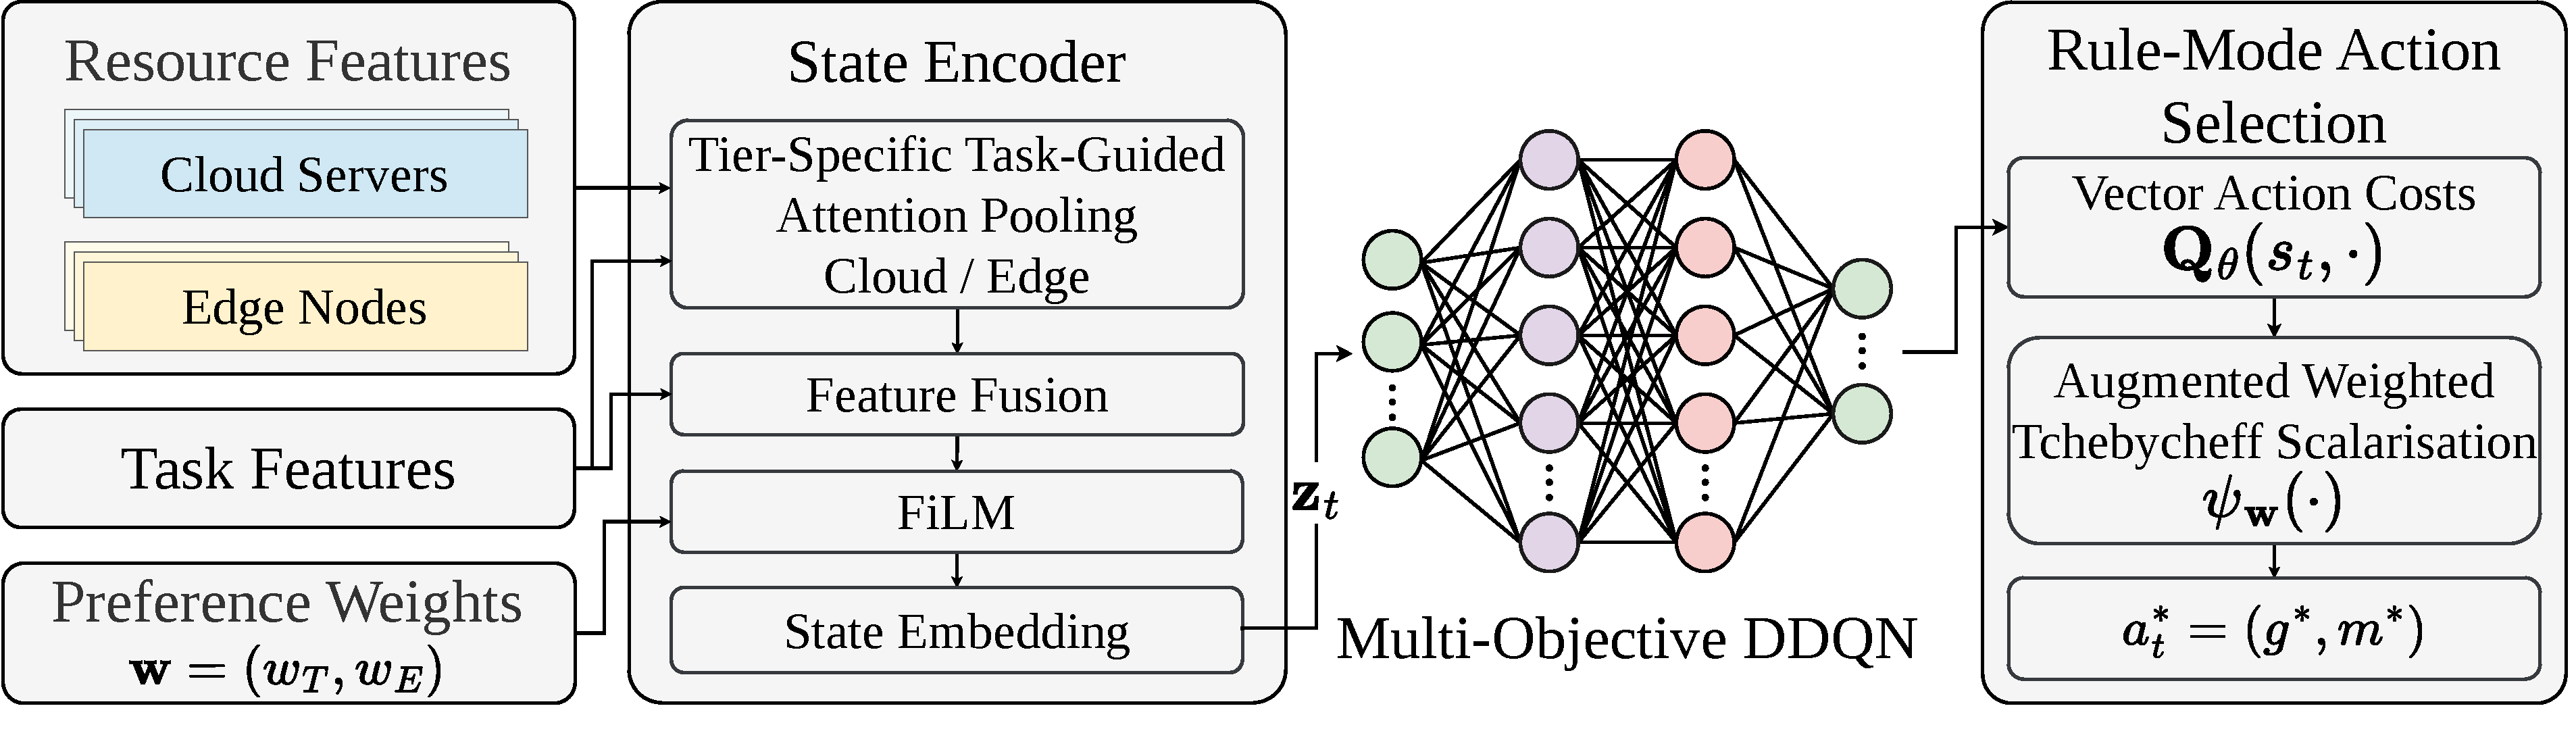
\includegraphics[width=0.78\textwidth]{figures/DRL.pdf}
\caption{Multi-objective DDQN for rule-mode action selection in PRS-GPDRL.}
\label{Fig: PRS-GPDRL DDQN}
\end{figure*}

Let $\mathbf{x}_t^{\mathrm{task}}$, $\mathbf{X}_t^{\mathrm{res}}$, and $\mathbf{w}$ denote the task features, feasible-resource features, and preference vector, respectively. Continuous task and resource attributes use signed logarithmic scaling, while categorical indicators remain unchanged. The task encoder contains two 64-unit layers with exponential linear unit (ELU) activations. For each resource tier, two 64-unit ELU layers produce key representations, and a 64-dimensional linear projection produces value representations. Single-head masked scaled dot-product attention uses the task embedding as the query and the resource keys to aggregate each tier into a 64-dimensional representation. The task and two tier-level representations are then fused by two 128-unit layers, with an ELU activation after the first, to produce $\mathbf{h}_{\mathrm{fuse}}\in\mathbb{R}^{128}$.

A FiLM layer \cite{perez2018film} conditions the fused representation on the preference. A preference multilayer perceptron (MLP) with a 32-unit ELU hidden layer outputs 256 values, which are split into 128-dimensional raw scale and shift vectors. The scale is parameterized as
$\boldsymbol{\gamma}_{\mathrm{film}}(\mathbf{w})=
1+0.3\tanh(\widetilde{\boldsymbol{\gamma}}_{\mathrm{film}}(\mathbf{w}))$,
which bounds its elements to $[0.7,1.3]$, while the shift remains unconstrained. This bound prevents sign reversal and excessive amplification in the multiplicative modulation. The FiLM transformation is
\begin{equation}
    \mathbf{z}_t =
    \boldsymbol{\gamma}_{\mathrm{film}}(\mathbf{w})\odot
    \mathbf{h}_{\mathrm{fuse}}
    +\boldsymbol{\delta}_{\mathrm{film}}(\mathbf{w}),
    \label{Eq: film state embedding}
\end{equation}
where $\boldsymbol{\gamma}_{\mathrm{film}}(\mathbf{w})$ and
$\boldsymbol{\delta}_{\mathrm{film}}(\mathbf{w})$ are preference-dependent scale
and shift vectors.

The 128-dimensional embedding $\mathbf{z}_t$ is processed by a shared 256--128 ReLU MLP and a linear output layer that produces a two-dimensional cost estimate for every rule-mode action:
\begin{equation}
    \mathbf{Q}_{\theta}(s_t,a) =
    \left(Q_{\theta}^{T}(s_t,a), Q_{\theta}^{E}(s_t,a)\right),
    \quad a\in\mathcal{A}.
    \label{Eq: vector Q}
\end{equation}
where $Q_{\theta}^{T}$ and $Q_{\theta}^{E}$ estimate cumulative tardiness-related and scaled energy costs, respectively.

Because lower values are better for both objectives, action selection minimizes an augmented weighted Tchebycheff cost. For state $s$, let $q_{\theta}^{j,\min}(s)=\min_{a'\in\mathcal{A}}Q_{\theta}^{j}(s,a')$, where $j\in\{T,E\}$. The scalarized cost is
\begin{equation}
\begin{aligned}
    \psi_{\mathbf{w}}\!\left(\mathbf{Q}_{\theta}(s,a)\right)
    ={}&\max_{j\in\{T,E\}}
    w_j\!\left(Q_{\theta}^{j}(s,a)-q_{\theta}^{j,\min}(s)\right)\\
    &+\zeta\sum_{j\in\{T,E\}}
    w_j\!\left(Q_{\theta}^{j}(s,a)-q_{\theta}^{j,\min}(s)\right),
\end{aligned}
    \label{Eq: tchebycheff scalarization}
\end{equation}
where $\zeta$ is the augmentation coefficient. The same scalarization is used for preference-specific DDQN updates and greedy action selection:
\begin{equation}
    a_t^{*} = \arg\min_{a\in\mathcal{A}}
    \psi_{\mathbf{w}}\left(\mathbf{Q}_{\theta}(s_t,a)\right).
    \label{Eq: greedy action}
\end{equation}


The DDQN is trained with experience replay and a periodically updated target network \cite{vanhasselt2016}. At the start of each training episode, a preference vector is sampled as follows:
\begin{equation}
    w_T\in\{0,0.05,\ldots,0.95,1\},
    \qquad w_E=1-w_T,
    \label{Eq: evaluation preference grid}
\end{equation}
The sampled preference is included in the state and fixed throughout the episode, so the network observes different tardiness--energy trade-offs during training. Checkpoint validation evaluates each validation episode under all 21 grid preferences. For preference $\mathbf{w}$, the cumulative validation cost is
$C^{\mathrm{val}}(\mathbf{w})=
w_T\sum_t\Delta T_t+w_E\kappa\sum_t\Delta E_t$.
The checkpoint with the lowest mean $C^{\mathrm{val}}(\mathbf{w})$ across the validation episodes and grid preferences is retained.

\subsection{Training and Inference Procedure}
\label{Sec: training inference}

After action extraction, training and testing are performed separately for each scenario $\langle\mathrm{wfNum},\lambda\rangle$ using its corresponding fixed rule pool and rule-mode action space. The DDQN learns from vector-cost transitions under sampled preferences using Eq.~\eqref{Eq: tchebycheff scalarization}, and the trained DDQN together with the fixed action space constitutes the PRS-GPDRL agent. During inference, upward-rank sequencing resolves simultaneous ready tasks when needed, after which the DDQN selects a rule-mode action and assigns the current task to the feasible resource with the minimum priority score.


\section{Experimental Design}
\label{Sec: experimental design}

\subsection{Experimental Setup}
\label{Sec: experimental environment}

We conduct the experiments using an event-driven simulator adapted from the workflow scheduling simulator in \cite{ccgp} to match the problem model in Section~\ref{Sec: problem modeling}.
Table~\ref{Table: resource configurations} lists five representative resource types for each tier. The configurations are derived from Amazon EC2\footnotemark[1], with CPU capacity measured in EC2 Compute Units (ECUs), and the power parameters follow the Teads model\footnotemark[2]. The Edge tier contains 19 fixed Edge Nodes, whereas Cloud Servers of the listed types can be provisioned on demand. Each task incurs a 50~ms container initialization delay \cite{Ranjan2020}, and provisioning a new Cloud Server takes 55.9~s. Following \cite{Goudarzi2021,Pallewatta2022}, the bandwidths of local-area and wide-area networks are set to 2.0 and 0.5~GB/s, and their communication latencies are 0.5 and 30~ms, respectively.

\begin{table*}[!t]
\caption{Configurations of Edge Nodes and Cloud Servers.}
\label{Table: resource configurations}
\centering
\begin{tabular}{@{}lrrrrlrrrr@{}}
\toprule
\multicolumn{5}{c}{Edge Nodes} & \multicolumn{5}{c}{Cloud Servers} \\
\cmidrule(lr){1-5}\cmidrule(lr){6-10}
\makecell{Type\\(number)} & ECU &
\makecell{CPU idle\\power (W)} &
\makecell{CPU full\\power (W)} &
\makecell{Base power\\(W)} &
Type & ECU &
\makecell{CPU idle\\power (W)} &
\makecell{CPU full\\power (W)} &
\makecell{Base power\\(W)} \\
\midrule
m1.small (3) & 1 & 0.72 & 5.76 & 1.2 &
m4.xlarge & 13 & 1.94 & 15.62 & 3.2 \\
m3.medium (3) & 3 & 0.87 & 6.97 & 1.4 &
m4.2xlarge & 26 & 3.89 & 31.24 & 6.4 \\
m3.large (4) & 6.5 & 1.73 & 13.94 & 2.9 &
m4.4xlarge & 53.5 & 7.77 & 62.47 & 12.9 \\
m3.xlarge (4) & 13 & 3.47 & 27.87 & 5.8 &
m4.10xlarge & 124.5 & 24.12 & 193.88 & 40.0 \\
m3.2xlarge (5) & 26 & 6.94 & 55.74 & 11.5 &
m4.16xlarge & 188 & 31.09 & 249.90 & 51.6 \\
\bottomrule
\end{tabular}
\vspace{-1em}
\end{table*}

Workflow templates are sampled from Alibaba Cluster-trace-v2018\footnotemark[3]. The public trace provides task dependencies and execution information, and the simulator reconstructs workflows from these data. Task input and output data sizes follow a discrete uniform distribution between 500 and 5000~MB. Each task is independently classified as CPU-sensitive or CPU-insensitive with equal probability. Workflow weights are independently sampled from $\{1,2,4\}$ with probabilities $0.2$, $0.6$, and $0.2$, respectively, following \cite{Hi2015ousgp}.
\footnotetext[1]{\url{https://aws.amazon.com/ec2/}}
\footnotetext[2]{\url{https://engineering.teads.com/sustainability/
carbon-footprint-estimator-for-aws-instances/}}
\footnotetext[3]{\url{https://github.com/alibaba/clusterdata}}

Workflow arrivals follow a Poisson process with rate $\lambda$, and the inter-arrival time is exponentially distributed with mean $1/\lambda$ \cite{Sahoo2021}. Following \cite{ccgp}, reference execution times and Edge transfer times are propagated along each DAG to obtain the largest earliest finish time $L_{\omega}$. The workflow deadline is set as $\rho^d(\omega)=\rho^a(\omega)+\delta_{\omega}L_{\omega}$, where the deadline factor $\delta_{\omega}$ is sampled uniformly from $\{0.8,1.0,1.5,1.8\}$.

Each scenario is denoted by $\langle\mathrm{wfNum},\lambda\rangle$, where $\mathrm{wfNum}$ is the total number of submitted workflows and $\lambda$ is the arrival rate. The main evaluation consists of the 12 combinations of $\mathrm{wfNum}\in\{10,15,20,30,50,100\}$ and $\lambda\in\{0.2,0.8\}$. For each scenario, 30 independent runs are conducted. In each run, every solution is evaluated on the same 30 unseen instances, and the objective values are averaged over these instances before the performance measures are calculated. The tables report the mean and standard deviation over the 30 runs.

\subsection{Compared Algorithms}
\label{Sec: compared methods}

Under the above experimental setting, the performance comparison includes CCGP, GATES, and LWFF, which represent GP hyper-heuristic, graph-based learning, and constructive heuristic methods, respectively. CCGP \cite{ccgp} coevolves task-sequencing, resource-selection, and container-scaling rules, and returns non-dominated scheduling heuristics. GATES \cite{gates} uses graph attention to encode ready tasks, workflow dependencies, and virtual machines, and learns an allocation policy through an evolution strategy. LWFF \cite{lwff} constructs non-dominated candidate resources and selects a resource according to resource waste and completion speed.

Because the original problem settings of these algorithms differ from the present model, necessary adaptations are made for a fair comparison. The adapted versions follow the experimental setup in Section~\ref{Sec: experimental environment} and use the objective definitions in Section~\ref{Sec: problem modeling}. For CCGP, task-sequencing and resource-selection rules are evolved, while the container-scaling rule is not used because CPU allocation is specified by Eq.~\eqref{Eq: cpu allocation}. For GATES, the learned policies are evaluated using weighted tardiness and energy consumption, and the final non-dominated policies form the approximation set. LWFF is evaluated on the same preference grid as PRS-GPDRL using upward-rank task sequencing and preference-weighted normalized estimates of weighted tardiness and energy.
The CCGP parameters follow \cite{ccgp} and are listed in Table~\ref{Table: CCGP parameters}. GATES uses a population of 100 policy networks and runs for 51 generations. The main DDQN and risk-stratified action augmentation parameters of PRS-GPDRL are listed in Table~\ref{Table: DDQN risk parameters}.

\begin{table}[!t]
\caption{Parameter settings of CCGP.}
\label{Table: CCGP parameters}
\centering
% \footnotesize
% \setlength{\tabcolsep}{5pt}
\begin{tabular}{cl}
\toprule
\textbf{Parameter} & \textbf{Value} \\
\midrule
Population size & 2 subpopulations of 50 \\
Number of generations & 51 \\
Method for initializing population & Ramped-half-and-half \\
Initial minimum/maximum depth & 2/7 \\
Elitism & 5 \\
Maximal depth & 8 \\
Crossover/mutation/reproduction rate & 0.80/0.15/0.05 \\
Terminal/non-terminal selection rate & 10\%/90\% \\
Environmental selection & \makecell[l]{Non-dominated Sorting\\Genetic Algorithm II (NSGA-II)} \\
\bottomrule
\end{tabular}
\end{table}

\begin{table}[!t]
\caption{Parameter settings of DDQN and risk-stratified action
augmentation.}
\label{Table: DDQN risk parameters}
\centering
% \footnotesize
% \setlength{\tabcolsep}{5pt}
\begin{tabular}{cl}
\toprule
\textbf{Parameter} & \textbf{Value} \\
\midrule
Training-step budget & $1{,}000{,}000$ \\
Exploration rate $\epsilon$ & 1.0 decays to 0.01 \\
Discount factor $\gamma$ & 1.0 \\
Learning rate & $5\times10^{-5}$ \\
Optimizer & Adam \\
Mini-batch size & 256 \\
Replay memory size & 200,000 \\
Target-update frequency & 5,000 \\
DDQN hidden-layer sizes & 256/128 \\
Maximum resource-selection rule pool size $K$ & 5 \\
Maximum risk mixing $\beta_{\max}$ & 0.75 \\
Energy-cost scaling $\kappa$ & $4.7\times10^5$ \\
Tchebycheff augmentation $\zeta$ & 0.05 \\
\bottomrule
\end{tabular}
\end{table}

\subsection{Performance Measures}
\label{Sec: evaluation metrics}

Each algorithm is evaluated by the approximation set it obtains in the weighted-tardiness--energy objective space. PRS-GPDRL and LWFF generate schedules over the preference grid in Eq.~\eqref{Eq: evaluation preference grid}, while CCGP and GATES use their final non-dominated heuristics or policies. For each method, dominated solutions are removed before calculating the performance measures.

HV and IGD are used as the performance measures for approximation sets. HV measures the dominated area of an approximation set and reflects both convergence and spread, while IGD measures the average distance from a reference set to the approximation set. Larger HV and smaller IGD indicate better performance. Before calculating HV and IGD, all solutions obtained by the algorithms in the same run are pooled, and each objective is min--max normalized:
\begin{equation}
    \widehat{f}_j(x)=
    \frac{f_j(x)-f_j^{\min}}
    {f_j^{\max}-f_j^{\min}},
    \label{Eq: objective normalization}
\end{equation}
where $f_j^{\min}$ and $f_j^{\max}$ are the minimum and maximum values of objective $f_j\in\{\mathbb{T},\mathbb{E}\}$ among the pooled solutions. HV is computed with the reference point $(1,1)$. Since the true Pareto front is unknown, the IGD reference set $Q$ is formed by the jointly non-dominated normalized solutions obtained in the same run. For an approximation set $P$, IGD is calculated as
\begin{equation}
    \operatorname{IGD}(P,Q)=
    \frac{1}{|Q|}
    \sum_{q\in Q}
    \min_{p\in P}\lVert p-q\rVert_2.
    \label{Eq: IGD}
\end{equation}

For each scenario and metric, statistical comparisons are performed using the Iman--Davenport-corrected Friedman test and two-sided paired Wilcoxon signed-rank tests at the 0.05 significance level. In the result tables, the arrows indicate that a result is statistically better ($\uparrow$), worse ($\downarrow$), or similar ($\approx$) compared with the preceding methods. W/D/L summarizes the number of scenarios in which the reported method is statistically better than, similar to, or worse than the reference method in the corresponding comparison. AverageRank reports the mean rank over the 30 runs, and a smaller value is better.

\section{Experimental Results}
\label{Sec: experimental results}

This section first reports the ablation study and diagnostic comparisons, and then compares the overall performance of PRS-GPDRL with the baselines.

\subsection{Ablation Study}
\label{Sec: ablation design analysis}

Table~\ref{Table: combined ablation results} reports the HV and IGD results of PRS-GPDRL and its three ablation variants in six representative scenarios. The \emph{w/o Risk} and \emph{w/o FiLM} variants remove the two components separately, while $K=3$ sets the maximum resource-selection rule pool size to three. All variants follow the same training, evaluation, and statistical analysis protocol.

\begin{table*}[!t]
\caption{The mean and standard deviation of the HV and IGD values for PRS-GPDRL
and its ablation variants over 30 independent runs.}
\label{Table: combined ablation results}
\centering
% \scriptsize
\setlength{\tabcolsep}{1.25pt}
\resizebox{\textwidth}{!}%
{\begin{tabular}{@{}lcccccccc@{}}
\toprule
\multirow{2}{*}{$\langle\mathrm{wfNum},\lambda\rangle$}
& \multicolumn{4}{c}{HV} & \multicolumn{4}{c}{IGD} \\
\cmidrule(lr){2-5}\cmidrule(lr){6-9}
& w/o Risk & w/o FiLM & $K=3$ & PRS-GPDRL
& w/o Risk & w/o FiLM & $K=3$ & PRS-GPDRL \\
\midrule
$\langle10,0.2\rangle$
& 0.833$\pm$0.095 & 0.851$\pm$0.074($\approx$) & 0.861$\pm$0.071($\uparrow$)($\uparrow$) & 0.868$\pm$0.067($\uparrow$)($\uparrow$)($\approx$)
& 0.083$\pm$0.045 & 0.060$\pm$0.031($\uparrow$) & 0.055$\pm$0.033($\uparrow$)($\approx$) & 0.049$\pm$0.026($\uparrow$)($\uparrow$)($\approx$) \\
$\langle10,0.8\rangle$
& 0.827$\pm$0.093 & 0.855$\pm$0.068($\uparrow$) & 0.880$\pm$0.064($\uparrow$)($\uparrow$) & 0.882$\pm$0.059($\uparrow$)($\uparrow$)($\approx$)
& 0.080$\pm$0.048 & 0.059$\pm$0.031($\uparrow$) & 0.042$\pm$0.019($\uparrow$)($\uparrow$) & 0.046$\pm$0.022($\uparrow$)($\uparrow$)($\approx$) \\
$\langle30,0.2\rangle$
& 0.814$\pm$0.103 & 0.848$\pm$0.074($\uparrow$) & 0.851$\pm$0.076($\approx$)($\approx$) & 0.867$\pm$0.060($\uparrow$)($\uparrow$)($\uparrow$)
& 0.090$\pm$0.055 & 0.066$\pm$0.046($\uparrow$) & 0.067$\pm$0.056($\uparrow$)($\approx$) & 0.054$\pm$0.046($\uparrow$)($\approx$)($\uparrow$) \\
$\langle30,0.8\rangle$
& 0.753$\pm$0.105 & 0.814$\pm$0.086($\uparrow$) & 0.809$\pm$0.080($\uparrow$)($\approx$) & 0.804$\pm$0.089($\uparrow$)($\approx$)($\approx$)
& 0.109$\pm$0.054 & 0.062$\pm$0.028($\uparrow$) & 0.072$\pm$0.033($\uparrow$)($\approx$) & 0.072$\pm$0.040($\uparrow$)($\approx$)($\approx$) \\
$\langle100,0.2\rangle$
& 0.778$\pm$0.117 & 0.828$\pm$0.075($\uparrow$) & 0.854$\pm$0.055($\uparrow$)($\uparrow$) & 0.847$\pm$0.077($\uparrow$)($\approx$)($\approx$)
& 0.115$\pm$0.071 & 0.082$\pm$0.046($\uparrow$) & 0.079$\pm$0.041($\uparrow$)($\approx$) & 0.078$\pm$0.039($\uparrow$)($\approx$)($\approx$) \\
$\langle100,0.8\rangle$
& 0.748$\pm$0.108 & 0.802$\pm$0.090($\uparrow$) & 0.816$\pm$0.080($\uparrow$)($\approx$) & 0.811$\pm$0.086($\uparrow$)($\approx$)($\approx$)
& 0.176$\pm$0.065 & 0.125$\pm$0.052($\uparrow$) & 0.121$\pm$0.050($\uparrow$)($\approx$) & 0.135$\pm$0.056($\uparrow$)($\approx$)($\approx$) \\
\midrule
W/D/L & 0/0/6 & 0/3/3 & 0/5/1 & N/A
      & 0/0/6 & 0/4/2 & 0/5/1 & N/A \\
AverageRank & 3.222 & 2.511 & 2.164 & 2.103
            & 3.350 & 2.356 & 2.247 & 2.047 \\
\bottomrule
\end{tabular}}
\end{table*}

\subsubsection{Risk-Stratified Action Augmentation and FiLM Conditioning}

This ablation examines the effects of the risk mode and FiLM conditioning while keeping the retained GP rule pool and scalarization scheme unchanged. Across the six representative scenarios, \emph{w/o Risk} records 0/0/6 against PRS-GPDRL for both metrics, showing the largest degradation among the three variants. Each retained GP rule provides a resource ranking, while the risk mode applies a bounded local correction according to the current state and preference. The consistent losses after removing this mode support its contribution to the final performance.

The \emph{w/o FiLM} variant records 0/3/3 for HV and 0/4/2 for IGD. Since this variant still uses vector-valued action costs and augmented weighted Tchebycheff scalarization, preference information remains available in action evaluation. The results suggest that FiLM provides additional preference-dependent modulation, although it is not the only channel through which preference information affects rule-mode selection.

\subsubsection{Rule-Pool Size}

This ablation examines the sensitivity to the size of the retained resource-selection rule pool. The $K=3$ variant records 0/5/1 for both metrics and is statistically comparable to PRS-GPDRL in five of the six scenarios. This result indicates that a smaller pool can retain much of the performance when the two endpoint rules and the balanced anchor rule are preserved. The $K=5$ setting still obtains the best average ranks, which is consistent with using additional neighboring rules to cover nearby trade-off regions.

Taken together, the ablation results show different effects of the three design choices. The risk mode gives the clearest component-level contribution, FiLM adds preference-dependent modulation to the state representation, and the pool-size comparison indicates that performance is not determined by action count alone.

\subsubsection{Task-Sequencing and Resource-Selection Diagnostics}
\label{Sec: task sequencing design}

This diagnostic comparison examines how performance changes when either the task-sequencing or resource-selection component of CCGP is replaced by the corresponding component of the Heterogeneous Earliest Finish Time (HEFT) algorithm \cite{Topcuoglu2002}. Table~\ref{Table: combined GP task sequencing} reports two CCGP-based diagnostic comparisons across the 12 scenarios. CCGP-UR replaces the GP task-sequencing rule of CCGP with upward-rank sequencing, and CCGP-EFT replaces the GP resource-selection rule with the earliest-finish-time (EFT) criterion while retaining the GP task-sequencing rule.

\begin{table}[!t]
\caption{The mean and standard deviation of the HV and IGD values obtained using CCGP-EFT, CCGP-UR, and CCGP over 30 independent runs.}
\label{Table: combined GP task sequencing}
\centering
% \scriptsize
\setlength{\tabcolsep}{1.8pt}
\resizebox{\linewidth}{!}
{\begin{tabular}{@{}lcccccc@{}}
\toprule
\multirow{2}{*}{$\langle\mathrm{wfNum},\lambda\rangle$}
& \multicolumn{3}{c}{HV} & \multicolumn{3}{c}{IGD} \\
\cmidrule(lr){2-4}\cmidrule(lr){5-7}
& CCGP-EFT & CCGP-UR & CCGP & CCGP-EFT & CCGP-UR & CCGP \\
\midrule
$\langle10,0.2\rangle$ & 0.289$\pm$0.223 & 0.791$\pm$0.090($\uparrow$) & 0.791$\pm$0.090($\uparrow$)($\approx$) & 0.524$\pm$0.131 & 0.103$\pm$0.037($\uparrow$) & 0.102$\pm$0.035($\uparrow$)($\approx$) \\
$\langle10,0.8\rangle$ & 0.325$\pm$0.223 & 0.787$\pm$0.117($\uparrow$) & 0.788$\pm$0.113($\uparrow$)($\approx$) & 0.469$\pm$0.118 & 0.111$\pm$0.041($\uparrow$) & 0.110$\pm$0.038($\uparrow$)($\approx$) \\
$\langle15,0.2\rangle$ & 0.257$\pm$0.193 & 0.799$\pm$0.108($\uparrow$) & 0.800$\pm$0.113($\uparrow$)($\approx$) & 0.468$\pm$0.119 & 0.071$\pm$0.028($\uparrow$) & 0.070$\pm$0.031($\uparrow$)($\approx$) \\
$\langle15,0.8\rangle$ & 0.384$\pm$0.187 & 0.754$\pm$0.144($\uparrow$) & 0.753$\pm$0.143($\uparrow$)($\approx$) & 0.407$\pm$0.112 & 0.085$\pm$0.053($\uparrow$) & 0.083$\pm$0.050($\uparrow$)($\approx$) \\
$\langle20,0.2\rangle$ & 0.320$\pm$0.206 & 0.787$\pm$0.136($\uparrow$) & 0.789$\pm$0.133($\uparrow$)($\approx$) & 0.455$\pm$0.141 & 0.080$\pm$0.042($\uparrow$) & 0.079$\pm$0.043($\uparrow$)($\approx$) \\
$\langle20,0.8\rangle$ & 0.339$\pm$0.163 & 0.781$\pm$0.105($\uparrow$) & 0.778$\pm$0.107($\uparrow$)($\approx$) & 0.418$\pm$0.117 & 0.071$\pm$0.032($\uparrow$) & 0.073$\pm$0.034($\uparrow$)($\approx$) \\
$\langle30,0.2\rangle$ & 0.350$\pm$0.150 & 0.823$\pm$0.100($\uparrow$) & 0.823$\pm$0.101($\uparrow$)($\approx$) & 0.446$\pm$0.104 & 0.080$\pm$0.037($\uparrow$) & 0.082$\pm$0.038($\uparrow$)($\approx$) \\
$\langle30,0.8\rangle$ & 0.390$\pm$0.169 & 0.784$\pm$0.099($\uparrow$) & 0.788$\pm$0.091($\uparrow$)($\approx$) & 0.428$\pm$0.106 & 0.079$\pm$0.029($\uparrow$) & 0.079$\pm$0.029($\uparrow$)($\approx$) \\
$\langle50,0.2\rangle$ & 0.405$\pm$0.171 & 0.806$\pm$0.104($\uparrow$) & 0.808$\pm$0.103($\uparrow$)($\approx$) & 0.382$\pm$0.102 & 0.083$\pm$0.041($\uparrow$) & 0.080$\pm$0.040($\uparrow$)($\uparrow$) \\
$\langle50,0.8\rangle$ & 0.363$\pm$0.207 & 0.781$\pm$0.133($\uparrow$) & 0.785$\pm$0.132($\uparrow$)($\uparrow$) & 0.482$\pm$0.121 & 0.075$\pm$0.037($\uparrow$) & 0.074$\pm$0.038($\uparrow$)($\approx$) \\
$\langle100,0.2\rangle$ & 0.445$\pm$0.157 & 0.813$\pm$0.096($\uparrow$) & 0.817$\pm$0.096($\uparrow$)($\approx$) & 0.358$\pm$0.091 & 0.076$\pm$0.034($\uparrow$) & 0.073$\pm$0.032($\uparrow$)($\approx$) \\
$\langle100,0.8\rangle$ & 0.493$\pm$0.187 & 0.850$\pm$0.070($\uparrow$) & 0.852$\pm$0.066($\uparrow$)($\approx$) & 0.428$\pm$0.118 & 0.067$\pm$0.026($\uparrow$) & 0.066$\pm$0.024($\uparrow$)($\approx$) \\
\midrule
W/D/L & 0/0/12 & 0/11/1 & N/A & 0/0/12 & 0/11/1 & N/A \\
AverageRank & 3.000 & 1.564 & 1.436 & 3.000 & 1.556 & 1.444 \\
\bottomrule
\end{tabular}}
\end{table}

CCGP-UR records 0/11/1 against CCGP for both metrics and has close average ranks. In contrast, CCGP-EFT records 0/0/12 against CCGP for both metrics and has the worst average rank. This contrast indicates that replacing the GP resource-selection rule with the EFT criterion leads to a much larger performance loss than replacing the GP task-sequencing rule with upward-rank sequencing.

The diagnostic results are consistent with the decision structure considered in this work. VMs can execute multiple tasks concurrently, resource selection is required for every dispatched task, and task sequencing is only needed when more than one task is ready at the same decision point. Moreover, treating task-sequencing rules as additional learned actions would introduce combinations of task-sequencing and resource-selection choices, which can increase training cost and may make policy learning more difficult. Thus, these results support the design choice in Section~\ref{Sec: PRS-GPDRL overall}: PRS-GPDRL retains upward-rank sequencing for ready-task sequencing and concentrates the learned action space on resource selection. They do not imply that task sequencing is unimportant in general, but indicate that it is not the main source of performance difference in the evaluated scenarios.

\subsection{Overall Performance}
\label{Sec: overall performance}
% The overall comparison examines whether PRS-GPDRL improves the quality of the obtained approximation sets over representative GP hyper-heuristic, graph-based learning, and constructive heuristic baselines. 
Table~\ref{Table: main results} presents the mean and standard deviation of the HV and IGD values over the 30 independent runs of the compared algorithms.
PRS-GPDRL obtains the best HV average rank (1.406), while CCGP records 1/1/10 relative to it. PRS-GPDRL is statistically better than or comparable to CCGP throughout $\mathrm{wfNum}\leq 50$, with clear gains in several small- and medium-scale scenarios. At $\mathrm{wfNum}=100$, PRS-GPDRL is better than CCGP at $\langle100,0.2\rangle$ but worse at $\langle100,0.8\rangle$, indicating that its advantage is less consistent under the largest workflow count with the higher arrival rate.

\begin{table*}[!t]
\caption{The mean and standard deviation of the HV and IGD values over the 30
independent runs of the compared algorithms.}
\label{Table: main results}
\centering
% \scriptsize
\setlength{\tabcolsep}{1.6pt}
\resizebox{\textwidth}{!}%
{\begin{tabular}{@{}lcccccccc@{}}
\toprule
\multirow{2}{*}{$\langle\mathrm{wfNum},\lambda\rangle$}
& \multicolumn{4}{c}{HV} & \multicolumn{4}{c}{IGD} \\
\cmidrule(lr){2-5}\cmidrule(lr){6-9}
& GATES & LWFF & CCGP & PRS-GPDRL
& GATES & LWFF & CCGP & PRS-GPDRL \\
\midrule
$\langle10,0.2\rangle$
& 0.535$\pm$0.185 & 0.599$\pm$0.128($\approx$) & 0.791$\pm$0.090($\uparrow$)($\uparrow$) & 0.868$\pm$0.067($\uparrow$)($\uparrow$)($\uparrow$)
& 0.310$\pm$0.128 & 0.226$\pm$0.077($\uparrow$) & 0.102$\pm$0.035($\uparrow$)($\uparrow$) & 0.049$\pm$0.026($\uparrow$)($\uparrow$)($\uparrow$) \\
$\langle10,0.8\rangle$
& 0.536$\pm$0.210 & 0.616$\pm$0.124($\uparrow$) & 0.788$\pm$0.113($\uparrow$)($\uparrow$) & 0.882$\pm$0.059($\uparrow$)($\uparrow$)($\uparrow$)
& 0.302$\pm$0.141 & 0.193$\pm$0.061($\uparrow$) & 0.110$\pm$0.038($\uparrow$)($\uparrow$) & 0.046$\pm$0.022($\uparrow$)($\uparrow$)($\uparrow$) \\
$\langle15,0.2\rangle$
& 0.567$\pm$0.124 & 0.603$\pm$0.105($\approx$) & 0.800$\pm$0.113($\uparrow$)($\uparrow$) & 0.862$\pm$0.087($\uparrow$)($\uparrow$)($\uparrow$)
& 0.247$\pm$0.093 & 0.158$\pm$0.050($\uparrow$) & 0.070$\pm$0.031($\uparrow$)($\uparrow$) & 0.045$\pm$0.030($\uparrow$)($\uparrow$)($\uparrow$) \\
$\langle15,0.8\rangle$
& 0.542$\pm$0.129 & 0.654$\pm$0.107($\uparrow$) & 0.753$\pm$0.143($\uparrow$)($\uparrow$) & 0.844$\pm$0.080($\uparrow$)($\uparrow$)($\uparrow$)
& 0.290$\pm$0.091 & 0.147$\pm$0.051($\uparrow$) & 0.083$\pm$0.050($\uparrow$)($\uparrow$) & 0.047$\pm$0.032($\uparrow$)($\uparrow$)($\uparrow$) \\
$\langle20,0.2\rangle$
& 0.608$\pm$0.166 & 0.633$\pm$0.121($\approx$) & 0.789$\pm$0.133($\uparrow$)($\uparrow$) & 0.869$\pm$0.087($\uparrow$)($\uparrow$)($\uparrow$)
& 0.251$\pm$0.124 & 0.165$\pm$0.075($\uparrow$) & 0.079$\pm$0.043($\uparrow$)($\uparrow$) & 0.050$\pm$0.045($\uparrow$)($\uparrow$)($\uparrow$) \\
$\langle20,0.8\rangle$
& 0.534$\pm$0.165 & 0.649$\pm$0.102($\uparrow$) & 0.778$\pm$0.107($\uparrow$)($\uparrow$) & 0.826$\pm$0.058($\uparrow$)($\uparrow$)($\uparrow$)
& 0.264$\pm$0.125 & 0.145$\pm$0.072($\uparrow$) & 0.073$\pm$0.034($\uparrow$)($\uparrow$) & 0.056$\pm$0.036($\uparrow$)($\uparrow$)($\approx$) \\
$\langle30,0.2\rangle$
& 0.635$\pm$0.139 & 0.675$\pm$0.091($\uparrow$) & 0.823$\pm$0.101($\uparrow$)($\uparrow$) & 0.867$\pm$0.060($\uparrow$)($\uparrow$)($\uparrow$)
& 0.238$\pm$0.107 & 0.145$\pm$0.051($\uparrow$) & 0.082$\pm$0.038($\uparrow$)($\uparrow$) & 0.054$\pm$0.046($\uparrow$)($\uparrow$)($\uparrow$) \\
$\langle30,0.8\rangle$
& 0.569$\pm$0.131 & 0.698$\pm$0.090($\uparrow$) & 0.788$\pm$0.091($\uparrow$)($\uparrow$) & 0.804$\pm$0.089($\uparrow$)($\uparrow$)($\approx$)
& 0.280$\pm$0.105 & 0.123$\pm$0.037($\uparrow$) & 0.079$\pm$0.029($\uparrow$)($\uparrow$) & 0.072$\pm$0.040($\uparrow$)($\uparrow$)($\approx$) \\
$\langle50,0.2\rangle$
& 0.611$\pm$0.152 & 0.702$\pm$0.098($\uparrow$) & 0.808$\pm$0.103($\uparrow$)($\uparrow$) & 0.851$\pm$0.114($\uparrow$)($\uparrow$)($\uparrow$)
& 0.227$\pm$0.090 & 0.109$\pm$0.040($\uparrow$) & 0.080$\pm$0.040($\uparrow$)($\uparrow$) & 0.059$\pm$0.043($\uparrow$)($\uparrow$)($\uparrow$) \\
$\langle50,0.8\rangle$
& 0.647$\pm$0.162 & 0.752$\pm$0.098($\uparrow$) & 0.785$\pm$0.132($\uparrow$)($\uparrow$) & 0.817$\pm$0.106($\uparrow$)($\uparrow$)($\uparrow$)
& 0.240$\pm$0.105 & 0.098$\pm$0.032($\uparrow$) & 0.074$\pm$0.038($\uparrow$)($\uparrow$) & 0.075$\pm$0.041($\uparrow$)($\uparrow$)($\approx$) \\
$\langle100,0.2\rangle$
& 0.579$\pm$0.192 & 0.697$\pm$0.090($\uparrow$) & 0.817$\pm$0.096($\uparrow$)($\uparrow$) & 0.847$\pm$0.077($\uparrow$)($\uparrow$)($\uparrow$)
& 0.262$\pm$0.133 & 0.139$\pm$0.060($\uparrow$) & 0.073$\pm$0.032($\uparrow$)($\uparrow$) & 0.078$\pm$0.039($\uparrow$)($\uparrow$)($\approx$) \\
$\langle100,0.8\rangle$
& 0.798$\pm$0.080 & 0.867$\pm$0.058($\uparrow$) & 0.852$\pm$0.066($\uparrow$)($\downarrow$) & 0.811$\pm$0.086($\approx$)($\downarrow$)($\downarrow$)
& 0.189$\pm$0.078 & 0.079$\pm$0.055($\uparrow$) & 0.066$\pm$0.024($\uparrow$)($\approx$) & 0.135$\pm$0.056($\uparrow$)($\downarrow$)($\downarrow$) \\
\midrule
W/D/L & 0/1/11 & 1/0/11 & 1/1/10 & N/A
      & 0/0/12 & 1/0/11 & 1/4/7 & N/A \\
AverageRank & 3.603 & 3.017 & 1.975 & 1.406
            & 3.792 & 2.828 & 1.894 & 1.486 \\
\bottomrule
\end{tabular}}
\end{table*}



PRS-GPDRL also obtains the best IGD average rank (1.486), with CCGP recording 1/4/7 relative to it. The IGD results follow a similar pattern: PRS-GPDRL is better than or comparable to CCGP throughout $\mathrm{wfNum}\leq 50$, whereas the two $\mathrm{wfNum}=100$ scenarios show mixed outcomes. GATES and LWFF are statistically better than PRS-GPDRL in at most one scenario for each metric, and their average ranks are higher than those of PRS-GPDRL and CCGP.

Because PRS-GPDRL extracts its resource-selection rule pool from the corresponding CCGP archive, the comparison with CCGP helps separate the source of GP rules from their online use. Together with the risk mode and $K=3$ ablations and the CCGP-UR/CCGP-EFT diagnostics, the results support the interpretation that preference-aware online selection of resource-selection rules and bounded local correction are important to the performance gain in the evaluated scenarios. The next section further examines the obtained trade-off profiles and the preference-dependent behavior of the learned policy.

\section{Further Analysis}
\label{Sec: further analysis}

This section further analyzes the obtained trade-off profiles and the behavior of the learned policy. The analysis focuses on whether PRS-GPDRL improves the distribution of non-dominated solutions and how the selected resource-selection rules and risk mode change with the requested preference.

\subsection{50\% Empirical Attainment Curves}

Fig.~\ref{Fig: tradeoff profiles} presents the 50\% empirical attainment curves
of the compared algorithms in the normalized weighted-tardiness--energy space
for six representative scenarios.

\begin{figure}[!t]
    \centering
    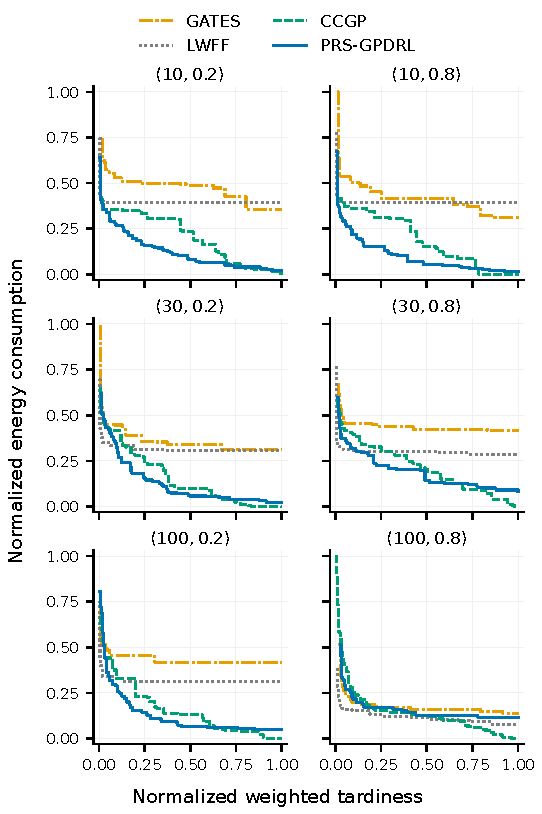
\includegraphics[width=.88\columnwidth]{figures/tradeoff_profile_50.pdf}
    \caption{The 50\% empirical attainment curves of the compared algorithms in
    six representative scenarios.}
    \label{Fig: tradeoff profiles}
\end{figure}

PRS-GPDRL lies below CCGP over most of their shared tardiness range in five panels, with the clearest separation in the two $\mathrm{wfNum}=10$ scenarios. Since the separation appears over the trade-off interior, the HV and IGD improvements are not limited to endpoint solutions.

\subsection{Objective Response to Preference}
\label{Sec: preference controllability}

Fig.~\ref{Fig: preference responses} shows the scenario-wise median relative
reductions in weighted tardiness and energy consumption as their corresponding
preference weights vary across the 12 scenarios. Let $x(w_j)$ denote the
solution obtained at objective weight $w_j$. For objective $f_j$, the relative
reduction is $[f_j(x(0))-f_j(x(w_j))]/f_j(x(0))$ from the endpoint at which its
own weight is zero.
Weighted tardiness is plotted against $w_T$, and energy against $w_E=1-w_T$.

\begin{figure*}[!t]
    \centering
    \begin{minipage}[t]{0.48\textwidth}
        \centering
        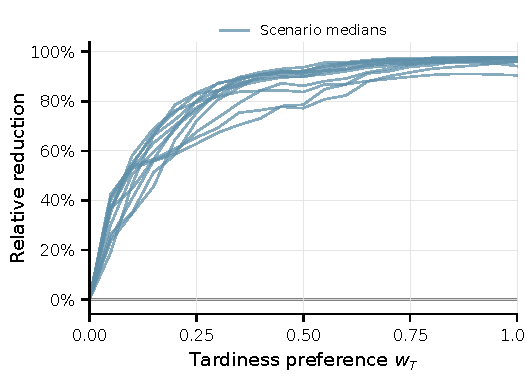
\includegraphics[width=.88\linewidth]{figures/preference_response_tardiness.pdf}
        \centerline{(a) Weighted tardiness response to $w_T$.}
    \end{minipage}\hfill
    \begin{minipage}[t]{0.48\textwidth}
        \centering
        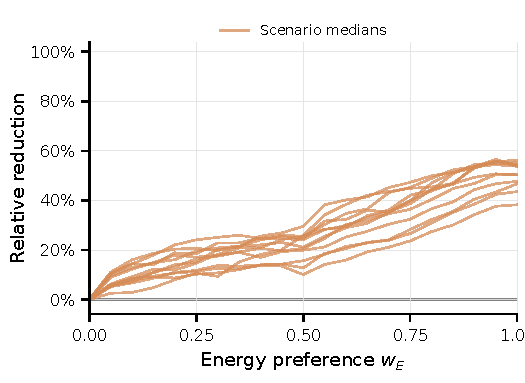
\includegraphics[width=.88\linewidth]{figures/preference_response_energy.pdf}
        \centerline{(b) Energy response to $w_E$.}
    \end{minipage}
    \caption{Relative reductions in weighted tardiness and energy consumption
    under different preference weights. Each curve shows the median over 30
    independent runs for one scenario.}
    \label{Fig: preference responses}
\end{figure*}

At the outcome level, increasing an objective's weight changes the schedule in the expected direction. Median reductions at weight 0.5 are 89.7\% for weighted tardiness and 20.5\% for energy. Over the full range, they reach 96.9\% and 51.1\%. The stronger response of weighted tardiness may be related to the threshold nature of tardiness penalties, where earlier completion near deadlines can sharply reduce the objective, whereas energy changes accumulate over resource active intervals.

The median correlations between each raw objective and its own weight are $\rho_T=-0.968$ and $\rho_E=-0.955$. All tardiness curves and 99.4\% of energy curves have the expected direction. In addition, 99.4\% of runs shift correctly between the endpoints. These results show that the learned policy generates preference-dependent scheduling outcomes across the tested preference grid.

\subsection{Preference-Dependent Resource-Selection Rule Usage}

Fig.~\ref{Fig: tree role frequency} shows how the use of the five retained
resource-selection rules varies with tardiness preference across the 12
scenarios. The rules are ordered from the minimum-energy endpoint to the
minimum-tardiness endpoint.

\begin{figure*}[!t]
    \centering
    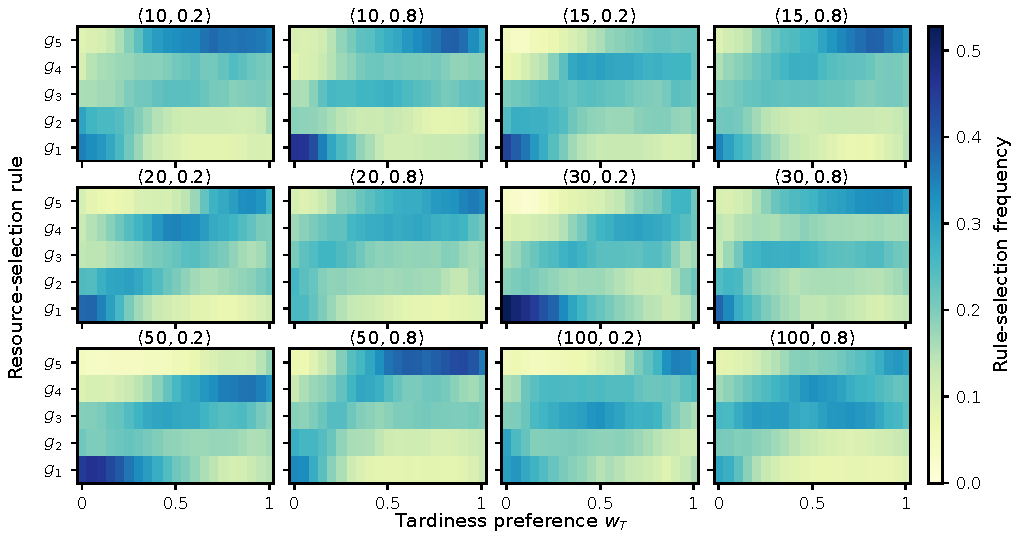
\includegraphics[width=.78\textwidth]{figures/tree_role_frequency.pdf}
    \caption{Mean selection frequencies over the included independent runs for
    each of the 12 scenarios under different tardiness preferences (runs
    retaining five rules). The roles are the minimum-energy endpoint $g_1$, its
    neighbor $g_2$, the balanced anchor $g_3$, the minimum-tardiness neighbor $g_4$, and
    the minimum-tardiness endpoint $g_5$.}
    \label{Fig: tree role frequency}
\end{figure*}

At the rule level, the minimum-energy rule and its neighbor account for 61.7\% of decisions at $w_T=0$, while the minimum-tardiness pair accounts for 50.3\% at $w_T=1$. The median weight--role correlation is $\rho_g=0.738$, and 90.4\% of included runs shift as expected. This pattern is consistent with Fig.~\ref{Fig: preference responses}: increasing $w_T$ moves rule selection from energy-oriented roles through the balanced anchor toward tardiness-oriented roles.

\subsection{Risk-Mode Usage}

Fig.~\ref{Fig: risk frequency} shows the risk-mode selection frequency as a
function of $w_T$ for the two arrival rates, with one panel for each workflow
count.

\begin{figure}[!t]
    \centering
    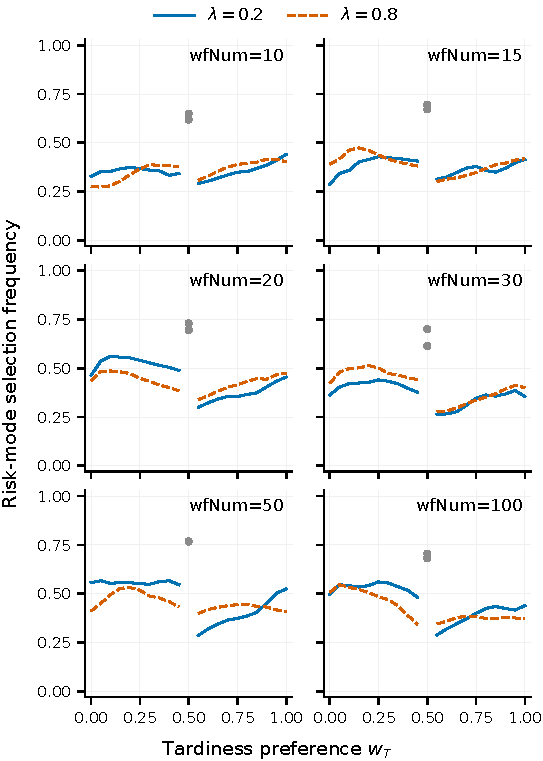
\includegraphics[width=.88\linewidth]{figures/risk_frequency.pdf}
    \caption{Mean risk-mode selection frequency over 30 independent runs for
    each of the 12 scenarios. Gray markers denote the balanced preference
    $w_T=w_E=0.5$. At the balanced preference, risk-mode
    selections are counted although their priority scores coincide with those
    of the base mode.}
    \label{Fig: risk frequency}
\end{figure}

At the mode level, the risk mode is selected in 42.5\% of decisions. Away from balance, non-zero correction is activated in 41.2\% of decisions, ranging from 26.1\% to 56.6\% across preferences and scenarios. These values indicate that the risk mode is used in a substantial fraction of decisions, while the remaining base-mode selections show that the unmodified GP ranking is still selected in many decisions.

Figs.~\ref{Fig: tree role frequency} and~\ref{Fig: risk frequency} describe two different levels of adaptation. Rule selection changes the main orientation of the resource ranking by moving from energy-oriented roles through the balanced anchor toward tardiness-oriented roles as $w_T$ increases. Risk-mode selection determines whether the selected rule should be locally corrected for the current decision. Its frequency does not need to vary monotonically with $w_T$, because the decision to apply correction can also depend on the current workflow and feasible-resource states.

Within the evaluated preference grid, the three figures analyze policy behavior at three levels. Fig.~\ref{Fig: preference responses} shows the objective response to preference changes, Fig.~\ref{Fig: tree role frequency} shows the corresponding change in resource-selection rule usage, and Fig.~\ref{Fig: risk frequency} shows when local correction is selected. Taken together, these observations indicate that preference conditioning is reflected in both the obtained objective values and the online decisions used to generate them.

\section{Conclusion}
\label{Sec: conclusion}

This paper proposes PRS-GPDRL for preference-aware online scheduling of
dynamic workflows in heterogeneous Cloud--Edge systems. PRS-GPDRL combines
CCGP-based rule discovery with multi-objective deep reinforcement learning:
a quality- and behavior-aware procedure extracts a compact pool of evolved
resource-selection rules, and a preference-conditioned DDQN adaptively selects
rule-mode actions according to the current scheduling state and requested
tardiness--energy trade-off. Experimental results show that PRS-GPDRL achieves
the best overall HV and IGD performance among the compared methods. The behavioral, ablation, and diagnostic analyses further indicate that complementary GP rules, preference conditioning, and state-dependent local correction are important to its adaptive scheduling performance. They also show that fixed upward-rank sequencing remains close to GP-based task sequencing in most scenarios, while the diagnostic comparison highlights the importance of GP-based resource selection in the evaluated setting.

The current framework still relies on an offline fixed rule pool, fixed
upward-rank task sequencing, and a predefined CPU-sharing mechanism. Future work
will investigate continual GP--DRL integration to update the rule pool during
deployment, hierarchical or multi-timescale learning for adaptive task sequencing
and resource selection, and fine-grained CPU allocation that dynamically
determines task-level CPU shares according to task characteristics, system
states, and scheduling preferences.

\bibliographystyle{IEEEtran}
\bibliography{Bibliography}

\end{document}
